\RequirePackage{fix-cm}
\documentclass[oneside]{report}

% Compiled with XeLaTeX + BibTeX or Tectonic.
\usepackage[no-math]{fontspec}
\newcommand{\ThesisTitle}{Longitudinal Learning with Tensor Fusion for Predicting Progression of Alzheimer’s Disease}
\newcommand{\ThesisTitleVN}{Học trên dữ liệu theo dõi dọc với hợp nhất tensor để dự đoán tiến triển bệnh Alzheimer}
\title{\ThesisTitle}
\author{Nguyen Phuong Nam}
\date{2026}

\setmainfont{LibertinusSerif}[
  Extension=.otf,
  UprightFont=*-Regular,
  BoldFont=*-Semibold,
  ItalicFont=*-Italic,
  BoldItalicFont=*-SemiboldItalic
]

\usepackage[a4paper,left=30mm,right=20mm,top=20mm,bottom=25mm]{geometry}
\usepackage{graphicx}
\usepackage{pdflscape}
\graphicspath{{image/}{figures/}}
\usepackage{tikz}
\usetikzlibrary{arrows.meta,positioning,calc,fit,backgrounds,shapes.geometric,matrix}
\usepackage{xcolor}
\definecolor{uetblue}{HTML}{0B4F78}
\definecolor{softblue}{HTML}{DCEEFF}
\definecolor{softgreen}{HTML}{E2F3E7}
\definecolor{softorange}{HTML}{FCE8D5}
\definecolor{softpurple}{HTML}{EAE2F3}
\definecolor{softgray}{HTML}{F3F4F6}
\definecolor{darkgreen}{HTML}{247A3C}
\definecolor{darkorange}{HTML}{B85C00}

\usepackage{amsmath,mathtools}
\usepackage[noOT1]{newtxmath}
\usepackage{bm}
\usepackage{booktabs,tabularx,longtable,multirow,array}
\usepackage{float}
\floatstyle{ruled}
\newfloat{algorithm}{htbp}{loa}
\floatname{algorithm}{Algorithm}
\floatstyle{plain}
\usepackage{caption}
\usepackage{subcaption}
\captionsetup{font=normalsize,labelfont=normalfont,textfont=normalfont,skip=6pt}
\usepackage{enumitem}
\usepackage{listings}
\usepackage{microtype}
\usepackage{scrextend}
\usepackage{indentfirst}
\usepackage{titlesec}
\usepackage{tocloft}
\usepackage{xurl}
\usepackage{csquotes}

\usepackage[numbers,sort&compress]{natbib}
\usepackage{placeins}
\usepackage{needspace}

\usepackage{hyperref}
\hypersetup{
  colorlinks=true,
  linkcolor=blue,
  citecolor=blue,
  urlcolor=blue,
  pdftitle={\ThesisTitle},
  pdfauthor={Nguyen Phuong Nam},
  pdfsubject={Longitudinal multimodal survival prediction with RC-Free CP-factorized pairwise fusion},
  pdfkeywords={Alzheimer, MCI, longitudinal learning, tensor fusion, CP, survival analysis}
}

\changefontsizes{13pt}
\renewcommand{\baselinestretch}{1.30}
\setlength{\parindent}{1cm}
\setlength{\parskip}{4pt}
\setlist{leftmargin=1cm,itemsep=0.2em,topsep=0.3em}
\titlespacing*{\section}{0pt}{0.8\baselineskip}{0.35\baselineskip}
\titlespacing*{\subsection}{0pt}{0.65\baselineskip}{0.25\baselineskip}
\titlespacing*{\subsubsection}{0pt}{0.5\baselineskip}{0.2\baselineskip}

\titleformat{\chapter}[display]{\normalfont\bfseries\huge}{\chaptername\ \thechapter}{8pt}{\Huge}
\titlespacing*{\chapter}{0pt}{0pt}{18pt}
\renewcommand{\chaptername}{Chapter}
\renewcommand{\contentsname}{TABLE OF CONTENTS}
\renewcommand{\listfigurename}{LIST OF FIGURES}
\renewcommand{\listtablename}{LIST OF TABLES}
\renewcommand{\figurename}{Figure}
\renewcommand{\tablename}{Table}

\renewcommand{\cftchappresnum}{Chapter~}
\renewcommand{\cftchapleader}{\normalfont\cftdotfill{\cftdotsep}}
\settowidth{\cftchapnumwidth}{Chapter~10\quad}
\renewcommand{\cftfigpresnum}{Figure~}
\settowidth{\cftfignumwidth}{Figure~10.10\quad}
\renewcommand{\cfttabpresnum}{Table~}
\settowidth{\cfttabnumwidth}{Table~10.10\quad}
\settowidth{\cftsecnumwidth}{10.10\quad}
\settowidth{\cftsubsecnumwidth}{10.10.10\quad}

\newcolumntype{L}[1]{>{\raggedright\arraybackslash}p{#1}}
\newcolumntype{C}[1]{>{\centering\arraybackslash}p{#1}}
\newcolumntype{R}[1]{>{\raggedleft\arraybackslash}p{#1}}
\newcolumntype{Y}{>{\raggedright\arraybackslash}X}
\newcommand{\R}{\mathbb{R}}
\newcommand{\T}{\mathsf{T}}
\newcommand{\Had}{\odot}
\newcommand{\concat}{\mathbin{\|}}
\newcommand{\softplus}{\operatorname{softplus}}
\newcommand{\LN}{\operatorname{LN}}
\newcommand{\MLP}{\operatorname{MLP}}
\newcommand{\diag}{\operatorname{diag}}
\newcommand{\sigmoid}{\operatorname{sigmoid}}

\lstdefinestyle{pythonstyle}{
  language=Python,
  basicstyle=\ttfamily\small,
  keywordstyle=\color{blue}\bfseries,
  commentstyle=\color{gray},
  stringstyle=\color{darkorange},
  breaklines=true,
  frame=single,
  backgroundcolor=\color{softgray},
  columns=fullflexible,
  showstringspaces=false
}

\setlength{\emergencystretch}{2em}
\clubpenalty=10000
\widowpenalty=10000
\displaywidowpenalty=10000

\newcommand{\bestresult}[1]{\textbf{\boldmath #1}}

\providecommand{\doi}[1]{\href{https://doi.org/#1}{DOI: \nolinkurl{#1}}}
\newcommand{\thesisurl}[1]{\url{#1}}
\renewcommand{\topfraction}{0.90}
\renewcommand{\bottomfraction}{0.85}
\renewcommand{\textfraction}{0.08}
\renewcommand{\floatpagefraction}{0.72}
\setcounter{topnumber}{3}
\setcounter{bottomnumber}{2}
\setcounter{totalnumber}{5}

\begin{document}
\special{pdf:minorversion 7}
\nocite{aghajanian2025longitudinal}

\hypersetup{pageanchor=false}
% Three covers follow the final Trang reference PDF, including its double frame.
\newcommand{\ThesisCoverFrame}{%
  \begin{tikzpicture}[overlay,remember picture]
    \draw[line width=3pt] ($(current page.north west)+(2.0cm,-2.0cm)$) rectangle ($(current page.south east)+(-1.5cm,1.8cm)$);
    \draw[line width=1pt] ($(current page.north west)+(2.15cm,-2.15cm)$) rectangle ($(current page.south east)+(-1.65cm,1.95cm)$);
  \end{tikzpicture}%
}

\begin{titlepage}
\setlength{\parskip}{0.5em}
\ThesisCoverFrame
\begin{center}
  \vspace*{0cm}
  \large
  \textbf{VIETNAM NATIONAL UNIVERSITY, HANOI\\UNIVERSITY OF ENGINEERING AND TECHNOLOGY}

  \vspace{1.5cm}
  
\includegraphics[width=0.3\textwidth]{UET.png}

  \vspace{0.5cm}
  \Large
  \textbf{NGUYEN PHUONG NAM}

  \vspace{1.5cm}
  {\fontsize{16}{23}\selectfont
  \textbf{LONGITUDINAL LEARNING WITH TENSOR FUSION\\FOR PREDICTING PROGRESSION OF ALZHEIMER’S DISEASE}\par}

  \vspace{2.5cm}
  \large
  \textbf{BACHELOR THESIS}\\
  \textbf{Major}: Artificial Intelligence

  \vfill
  \textbf{HA NOI - 2026}
\end{center}
\end{titlepage}

\begin{titlepage}
\setlength{\parskip}{0.5em}
\ThesisCoverFrame
\begin{center}
  \vspace*{0cm}
  \large
  \textbf{ĐẠI HỌC QUỐC GIA HÀ NỘI\\TRƯỜNG ĐẠI HỌC CÔNG NGHỆ}

  \vspace{3cm}
  \Large
  \textbf{NGUYỄN PHƯƠNG NAM}

  \vspace{1.5cm}
  \Large
  \textbf{\MakeUppercase{\ThesisTitleVN}}

  \vspace{1.5cm}
  \large
  \textbf{KHÓA LUẬN TỐT NGHIỆP CỬ NHÂN}\\
  \textbf{Ngành}: Trí tuệ nhân tạo

  \vspace{1cm}
  \begin{flushleft}
  \hspace*{0.2cm}%
  \begin{tabular}{@{}l@{\hspace{0.4cm}}l@{}}
    \textbf{Cán bộ hướng dẫn}: & GS. TS. Nguyễn Linh Trung\\[0.7cm]
    \textbf{Cán bộ đồng hướng dẫn}: & TS. Nguyễn Thành Trung
  \end{tabular}
  \end{flushleft}

  \vfill
  \textbf{HÀ NỘI - 2026}
\end{center}
\end{titlepage}

\begin{titlepage}
\setlength{\parskip}{0.5em}
\ThesisCoverFrame
\begin{center}
  \vspace*{0cm}
  \large
  \textbf{VIETNAM NATIONAL UNIVERSITY, HANOI\\UNIVERSITY OF ENGINEERING AND TECHNOLOGY}

  \vspace{3cm}
  \Large
  \textbf{NGUYEN PHUONG NAM}

  \vspace{1.5cm}
  {\fontsize{16}{23}\selectfont
  \textbf{LONGITUDINAL LEARNING WITH TENSOR FUSION\\FOR PREDICTING PROGRESSION OF ALZHEIMER’S DISEASE}\par}

  \vspace{1.5cm}
  \large
  \textbf{BACHELOR THESIS}\\
  \textbf{Major}: Artificial Intelligence

  \vspace{1cm}
  \begin{flushleft}
  \hspace*{0.2cm}%
  \begin{tabular}{@{}l@{\hspace{0.4cm}}l@{}}
    \textbf{Supervisor}: & Prof. Nguyen Linh Trung\\[0.7cm]
    \textbf{Co-Supervisor}: & Dr. Nguyen Thanh Trung
  \end{tabular}
  \end{flushleft}

  \vfill
  \textbf{HA NOI - 2026}
\end{center}
\end{titlepage}

\clearpage
\hypersetup{pageanchor=true}

\pagenumbering{roman}
\setcounter{page}{3}
\titleformat{name=\chapter,numberless}[display]{\normalfont\bfseries\large\filcenter}{}{0pt}{}
\chapter*{TÓM TẮT}
\addcontentsline{toc}{chapter}{TÓM TẮT}

Suy giảm nhận thức nhẹ (MCI) có diễn biến lâm sàng rất khác nhau: một số người bệnh sớm chuyển biến thành sa sút trí tuệ do bệnh Alzheimer, trong khi nhiều người khác duy trì trạng thái ổn định qua nhiều năm. Khóa luận xây dựng quy trình học sâu phân tích sống còn đa phương thức nhằm xếp hạng nguy cơ tiến triển từ lịch sử ba lần thăm khám theo dõi dọc, kết hợp ba nguồn thông tin: ảnh cộng hưởng từ cấu trúc 3D (MRI), đặc trưng định lượng hình dạng và kết cấu trích từ ảnh (radiomics), cùng thang điểm nhận thức và chức năng lâm sàng (MMSE, CDR).

Về mặt kiến trúc, tôi đề xuất mô hình \textbf{RC-Free Pairwise Fusion (RC-Free)} mô hình hóa tường minh hai tương tác song tuyến theo cặp quanh ảnh MRI gồm MRI--Radiomics (MR) và MRI--Lâm sàng (MC), đồng thời lược bỏ tương tác trực tiếp giữa radiomics và lâm sàng (RC). Để tránh bùng nổ tham số trên cỡ mẫu y tế hạn chế, mỗi lớp tương tác song tuyến đầu được tham số hóa bằng phân rã tensor Canonical Polyadic (CP) hạng thấp, sau đó truyền ngược lại biểu diễn gốc của từng nguồn qua kết nối phần dư có cổng điều tiết. Qua ba lần khám có khoảng cách thời gian không đều, mạng T-LSTM và cơ chế chú ý (attention) tổng hợp chuỗi đặc trưng thành một biểu diễn dọc để mô hình Cox tính điểm log-nguy cơ.

Nghiên cứu đánh giá hồi cứu trên dữ liệu của 359 người tham gia từ ADNI (251 huấn luyện, 54 xác thực và 54 kiểm tra hậu nghiệm). Qua ba lần khởi tạo, RC-Free đạt chỉ số đồng thuận (C-index) xác thực trung bình $0.8347\pm0.0237$. Khi phân nhóm nguy cơ theo ngưỡng trung vị tập huấn luyện, hai đường cong Kaplan--Meier tách biệt có ý nghĩa thống kê (kiểm định log-rank, $p=0.0134$). Diện tích dưới đường cong ROC phụ thuộc thời gian (IPCW-AUC) tại 2, 3 và 5 năm lần lượt đạt $0.9805\pm0.0149$, $0.9788\pm0.0162$ và $0.7889\pm0.0632$, ứng với 7, 7 và 12 biến cố tích lũy.

Phân rã CP giúp giảm 98.38\% tổng số tham số của ba lớp song tuyến đầu. Trong bảy cấu trúc CP có tương tác cặp, RC-Free đạt C-index xác thực trung bình cao nhất (0.8347), tiết kiệm thêm 15460 tham số so với Full CP mà vẫn giữ đủ cả ba nguồn đầu vào.

\noindent\textbf{Từ khóa:} Bệnh Alzheimer, MCI, MRI dọc, radiomics, hợp nhất tensor CP, phân tích sống còn.

\chapter*{ABSTRACT}
\addcontentsline{toc}{chapter}{ABSTRACT}

Mild cognitive impairment (MCI) is a pivotal intermediate stage with heterogeneous clinical trajectories: while some individuals progress rapidly to Alzheimer's dementia, many others remain stable over several years. This thesis develops a multimodal deep survival pipeline to rank progression risk from three longitudinal follow-up visits by integrating 3D structural magnetic resonance imaging (MRI), quantitative shape and texture descriptors (radiomics), and clinical cognitive and functional scores (MMSE and CDR).

Architecturally, I propose \textbf{RC-Free Pairwise Fusion (RC-Free)} to explicitly model two MRI-centered bilinear pairwise interactions---MRI--Radiomics (MR) and MRI--Clinical (MC)---while omitting the direct Radiomics--Clinical (RC) interaction. To prevent parameter explosion on a modest medical cohort, each initial bilinear layer is parameterized via low-rank Canonical Polyadic (CP) tensor decomposition, and interaction features are routed back to enrich the original modality representations through dynamically gated residual connections. Across three irregularly spaced visits, a Time-Aware LSTM (T-LSTM) coupled with additive attention aggregates the visit sequence into a unified representation from which a Cox head estimates the log-risk score.

Retrospective evaluation on 359 ADNI participants (251 training, 54 validation, and 54 post-hoc test) yields a mean validation C-index of $0.8347\pm0.0237$ across three random initializations. Stratifying risk groups by the training-set median cutoff produces statistically separated Kaplan--Meier survival curves (log-rank $p=0.0134$). Time-dependent IPCW-AUCs at 2, 3, and 5 years reach $0.9805\pm0.0149$, $0.9788\pm0.0162$, and $0.7889\pm0.0632$, based on 7, 7, and 12 cumulative cases, respectively.

Applying CP decomposition reduces the parameter count of the three initial bilinear layers by 98.38\%. Across all seven surveyed CP architectures with pairwise interactions, RC-Free attains the highest mean validation C-index (0.8347), uses 15460 fewer parameters than Full CP, and preserves all three input modalities.

\noindent\textbf{Keywords:} Alzheimer's disease, MCI, longitudinal MRI, radiomics, CP tensor fusion, survival analysis.

\chapter*{ACKNOWLEDGEMENTS}
\addcontentsline{toc}{chapter}{ACKNOWLEDGEMENTS}

I would like to express my deepest gratitude to Prof. Dr. Nguyen Linh Trung and Senior Lieutenant Colonel, Dr. Nguyen Thanh Trung, Deputy Head of the Department of Medical Equipment at 108 Military Central Hospital. Their dedicated guidance, insightful critiques, and rigorous academic discussions helped me define my research direction, grasp the scientific requirements of this topic, and persevere in completing this thesis.

I extend my sincere appreciation to Ms. Nguyen Phuong Trang for her constant willingness to support, mentor, and exchange ideas with me throughout this work. Her constructive feedback and companionship helped me resolve numerous technical hurdles and sustained my motivation whenever the research became challenging.

I am also grateful to Mr. Sepehr Aghajanian, author of the reference study upon which this thesis builds, for generously taking the time to reply to my emails and clarify my technical inquiries. His openness deepened my understanding of the inherited methodology and reinforced my appreciation for knowledge sharing within the scientific community.

I gratefully acknowledge the Avitech Lab team for providing server computing resources for model training and experimentation, which was essential for carrying out the empirical evaluations of this study.

My heartfelt thanks go to the faculty of the University of Engineering and Technology, Vietnam National University, Hanoi, for providing me with a solid academic foundation. I also recognize the researchers, clinical sites, sponsors, and participants of the Alzheimer's Disease Neuroimaging Initiative (ADNI) for establishing and maintaining the dataset used in this research.

Finally, I owe my warmest gratitude to my family and loved ones for their unconditional love, trust, and enduring encouragement, which have been my strongest anchor through every challenge until the final lines of this thesis.

\chapter*{DECLARATION}
\addcontentsline{toc}{chapter}{DECLARATION}

I hereby declare that the contents presented in this thesis represent my own independent research and implementation conducted under the supervision of my advisors. All concepts, mathematical formulations, and findings adopted from existing literature have been explicitly cited in the reference list. The ADNI dataset was accessed and utilized in strict accordance with its applicable data use agreements and regulatory guidelines.

All empirical figures and quantitative metrics reported herein have been systematically cross-checked against archived configuration logs, fixed data partitions, and provenance records. I assume full responsibility for the integrity of the experimental results and for the accurate representation of the study's scope.

\vspace{1.5cm}
\begin{flushright}
\begin{tabular}{@{}c@{}}
Hanoi, 2026\\[1.5cm]
\textbf{Nguyen Phuong Nam}
\end{tabular}
\end{flushright}

\titleformat{name=\chapter,numberless}[display]{\normalfont\bfseries\Huge}{}{0pt}{}
\chapter*{LIST OF ABBREVIATIONS}
\addcontentsline{toc}{chapter}{LIST OF ABBREVIATIONS}

{\renewcommand{\baselinestretch}{1.10}\small
\renewcommand{\arraystretch}{1.0}
\begin{longtable}{@{}L{2.5cm}L{12.7cm}@{}}
\toprule
Abbreviation & Description \\
\midrule
\endhead
AD & Alzheimer's Disease \\
ADNI & Alzheimer's Disease Neuroimaging Initiative \\
AUC & Area Under the ROC Curve \\
BN & Batch Normalization \\
C-index & Concordance Index \\
CDR & Clinical Dementia Rating \\
CDR-SB & Clinical Dementia Rating Sum of Boxes (sum of scores across six CDR domains) \\
CI & Confidence Interval \\
CNN & Convolutional Neural Network \\
CP & CANDECOMP/PARAFAC (Canonical Polyadic) decomposition into a sum of rank-one tensors \\
FP16 / FP32 & 16-bit / 32-bit Floating-Point numerical precision \\
GELU & Gaussian Error Linear Unit activation function \\
GLCM & Gray-Level Co-occurrence Matrix \\
GLDM & Gray-Level Dependence Matrix \\
GLRLM & Gray-Level Run Length Matrix \\
GLSZM & Gray-Level Size Zone Matrix \\
GPU & Graphics Processing Unit \\
HR & Hazard Ratio \\
IBSI & Image Biomarker Standardization Initiative \\
IPCW & Inverse Probability of Censoring Weighting \\
LN & Layer Normalization \\
LSTM & Long Short-Term Memory network \\
MC & MRI--Clinical pairwise interaction between 3D MRI and clinical features \\
MCI & Mild Cognitive Impairment \\
MLP & Multi-Layer Perceptron \\
MMSE & Mini-Mental State Examination \\
MNI & Montreal Neurological Institute standard brain coordinate template \\
MR & MRI--Radiomics pairwise interaction between 3D MRI and radiomics features \\
MRI & Magnetic Resonance Imaging \\
NGTDM & Neighbouring Gray Tone Difference Matrix \\
NIA-AA & National Institute on Aging and Alzheimer's Association \\
PCA & Principal Component Analysis \\
PH & Proportional Hazards assumption \\
RAS & Right--Anterior--Superior standard anatomical axis orientation \\
RC & Radiomics--Clinical pairwise interaction between radiomics and clinical features \\
RC-Free & Pairwise fusion topology omitting the direct RC interaction while retaining MR and MC pairs \\
ReLU & Rectified Linear Unit activation function \\
RID & Research Identifier (unique participant identifier in the ADNI dataset) \\
ROC & Receiver Operating Characteristic curve \\
RQ & Research Question \\
SD & Sample Standard Deviation \\
T-LSTM & Time-Aware Long Short-Term Memory network accounting for irregular time intervals \\
\bottomrule
\end{longtable}\par
}

\clearpage

\setcounter{secnumdepth}{2}
\setcounter{tocdepth}{1}
\tableofcontents
\clearpage
\listoffigures
\clearpage
\listoftables
\clearpage

\pagenumbering{arabic}
\setcounter{page}{1}
\chapter{Introduction}
\label{chap:intro}

\section{Research Motivation}
Alzheimer's disease (AD) is currently the leading cause of dementia worldwide, progressively eroding memory, cognitive reasoning, and functional autonomy in daily living \cite{cdc2024alzheimers}. Prior to developing overt dementia, the majority of patients pass through a pivotal intermediate stage known as \emph{mild cognitive impairment} (MCI): at this stage, memory or specific cognitive faculties have declined noticeably relative to age-normative expectations, yet individuals retain independence across most basic daily activities and primarily experience difficulties with complex cognitive tasks \cite{jack2018niaaa}. Notably, the clinical trajectories of individuals with MCI are remarkably heterogeneous: some patients convert rapidly to dementia within a short period, whereas others remain clinically stable for many years or even exhibit cognitive improvement \cite{petersen2018mci}. Motivated by this clinical reality, this thesis addresses a core research question: \emph{Given the longitudinal clinical history of an individual with MCI, can we accurately rank whether that patient faces an earlier or later risk of progression?}

A single scan can support risk prediction, but measuring within-person anatomical change requires observations at more than one time point. Indeed, a single structural brain magnetic resonance imaging (MRI) scan only reflects anatomical morphology on the exact day of acquisition, much like a static photograph that cannot convey the velocity or trajectory of tissue degeneration. Conversely, tracking a sequence of repeated scans from the same individual over time provides the necessary foundation for a model to capture the rate of anatomical atrophy, such as the pace of hippocampal volume loss \cite{dong2021deepatrophy}. Crucially, in real-world clinical follow-up data, the time intervals between consecutive visits are not uniform but vary considerably across patients (Table~\ref{tab:baseline-characteristics}). Consequently, I employ a Time-Aware Long Short-Term Memory (T-LSTM) network, which incorporates the actual elapsed time intervals between consecutive visits directly into the recurrent state update equations \cite{baytas2017patient}.

Furthermore, at each clinical visit, this thesis does not rely solely on a single MRI modality but actively harnesses three deeply complementary sources of information:
\begin{enumerate}
\item \emph{3D structural magnetic resonance imaging (MRI)}: provides comprehensive anatomical coverage of the brain and captures macroscopic structural changes such as hippocampal atrophy or ventricular enlargement \cite{weiner2015impact}.
\item \emph{Radiomics features}: a collection of quantitative mathematical descriptors that directly measure spatial geometry, voxel intensity distributions, and the coarseness or fineness of brain tissue textures extracted from the MRI volume itself \cite{vangriethuysen2017computational}.
\item \emph{Clinical data}: quantitative scores from the Mini-Mental State Examination (MMSE) and the Clinical Dementia Rating (CDR) scale evaluating cognitive and functional decline \cite{folstein1975mmse,morris1993cdr}.
\end{enumerate}

Although these three data sources reflect the pathological state of the same individual from complementary perspectives, they differ fundamentally in physical nature, representational dimensionality, and signal-to-noise characteristics. Consequently, the strategy used to fuse them plays a decisive role in determining the model's prognostic accuracy. Specifically, in the study serving as the direct reference baseline for this thesis, Aghajanian et al. (2025) combined a convolutional neural network (CNN), principal component analysis (PCA), a T-LSTM, and an attention mechanism over longitudinal MRI sequences to estimate progression risk under a Cox proportional hazards survival framework \cite{aghajanian2025longitudinal}. However, under their exact T-LSTM with attention configuration (Table~2 of their paper), concatenating gray-matter radiomics features with CNN features caused the mean concordance index (C-index) to decrease slightly from 0.85 to 0.84 on the validation set and from 0.91 to 0.90 on the test set; for this reason, the authors excluded radiomics from their final model \cite{aghajanian2025longitudinal}. This empirical finding raises a compelling scientific question: \emph{Could the apparent lack of benefit from radiomics stem from the fact that simple feature concatenation fails to exploit cross-modal interactions across data sources?}

To address this question, this thesis inherits the prognostic task formulation and reference data framework of Aghajanian et al., but fundamentally redesigns the multimodal fusion mechanism. Rather than merely concatenating feature vectors side by side, I explicitly model bilinear interactions between pairs of modalities. Specifically, given three sources---MRI (M), radiomics (R), and clinical scores (C)---there are three candidate pairwise interactions: MRI--Radiomics (MR), MRI--Clinical (MC), and Radiomics--Clinical (RC). To thoroughly mitigate the risk of parameter explosion when computing cross-products on a modest medical cohort, each bilinear interaction layer is tightly compressed via \emph{low-rank Canonical Polyadic (CP) tensor decomposition} \cite{kolda2009tensor,liu2018lowrank}, and the resulting interaction signals are routed back to the original modality representations through dynamically gated residual connections. In particular, recognizing that radiomics features are derived directly from the MRI scan itself, I propose a streamlined architecture termed \textbf{RC-Free Pairwise Fusion (RC-Free)}: positioning MRI as the central hub connecting the MR and MC pairs while deliberately omitting the direct RC interaction. The validity and effectiveness of this architectural choice are rigorously verified through controlled empirical comparisons against all seven pairwise interaction topologies in Section~\ref{sec:new-topology}.

\section{Problem Formulation}
This thesis addresses the problem of building a deep survival model to rank progression risk among individuals with MCI using data from the Alzheimer's Disease Neuroimaging Initiative (ADNI) \cite{weiner2015impact}. The study cohort comprises 359 participants who completed three MRI scans within 18 months of their baseline visit; each scan is synchronously paired with its corresponding whole-brain radiomics feature vector and clinical assessment scores. The three scan dates $s_1<s_2<s_3=p\leq L$ form a longitudinal observation sequence with subject-specific inter-visit time intervals. From this sequence of three clinical visits, the proposed method estimates a scalar log-risk score $\eta_i\in\mathbb R$ for each individual to rank future cognitive decline risk: participants assigned a higher $\eta_i$ are predicted to experience earlier progression.

\begin{figure}[H]
\centering
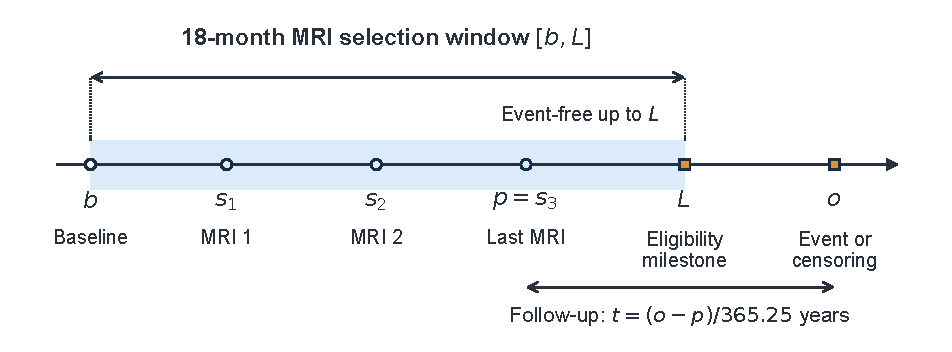
\includegraphics[width=\textwidth]{image_en/mci-progression-timeline.pdf}
\caption{Timeline of the longitudinal MCI progression prediction task}
\label{fig:problem-timeline}
\end{figure}

Figure~\ref{fig:problem-timeline} visually illustrates the temporal axis of the problem, clearly distinguishing the input observation window (three scans acquired at or before the cohort eligibility milestone $L$, defined as the baseline visit date plus 18 calendar months) from the post-$L$ clinical outcome follow-up period. To quantify cognitive and functional decline accurately, this thesis utilizes two well-established clinical rating scales:
\begin{enumerate}
\item \emph{MMSE (Mini-Mental State Examination)}: a 0-to-30 point scale evaluating global cognitive function, where lower scores indicate more severe cognitive impairment \cite{folstein1975mmse}.
\item \emph{CDR-global (global Clinical Dementia Rating)}: categorizes dementia severity into five levels---0 (normal), 0.5 (very mild dementia), 1 (mild), 2 (moderate), and 3 (severe)---according to the standardized scoring rules established by the scale's developers \cite{morris1993cdr,knightcdrscoring}.
\end{enumerate}

Inheriting the clinical convention of Aghajanian et al. \cite{aghajanian2025longitudinal}, a \emph{progression event} in this study is recorded at the first follow-up visit after milestone $L$ that satisfies either MMSE $<24$ or CDR-global $\geq1$. This constitutes a score-threshold-defined clinical event. Over long-term longitudinal follow-up, many participants withdraw from the study or reach the end of the observation period without ever crossing this threshold; consequently, their subsequent disease status remains unknown, except for the confirmed fact that they remained stable up to their last recorded visit. This statistical phenomenon is referred to as \emph{right-censoring}. Rather than forcing the task into a binary Yes/No classification paradigm (which would inevitably require discarding or mislabeling censored participants), this thesis formulates the problem within a \emph{survival analysis} framework to fully and equitably leverage both censoring status and actual follow-up duration.

Furthermore, from a methodological standpoint, a crucial detail in the time-axis definition must be noted: the survival model measures follow-up time starting from the third MRI scan date $p$, whereas the cohort inclusion criteria require participants to remain event-free through the 18-month milestone $L$. Whenever $p<L$, the interval between $p$ and $L$ is guaranteed to be event-free by virtue of the cohort selection rule itself, inducing \emph{immortal time bias} \cite{suissa2008immortal} if the model were interpreted as a prospective forecasting tool deployed immediately on scan date $p$. Accordingly, all empirical results in this thesis are carefully interpreted for the retrospective risk-ranking task among participants confirmed to have remained stable up to milestone $L$ (analyzed in detail in Sections~\ref{sec:study-design} and~\ref{sec:study-limitations}).

\section{Technical Challenges and Research Scope}
Developing a multimodal deep survival model over longitudinal medical sequences poses three primary technical challenges:
\begin{enumerate}
\item \emph{Balancing interaction expressiveness against parameter capacity}: Concatenating feature vectors introduces no additional parameters at the fusion step, but fails to explicitly construct second-order cross-products across modalities. Conversely, the outer product captures all bilinear interactions exhaustively, yet causes the weight count of the subsequent linear projection layer to grow multiplicatively with input and output dimensions \cite{zadeh2017tensor,liu2018lowrank}, easily triggering severe overfitting when the training set contains only 251 patients. While CP tensor decomposition substantially compresses the weight count via low-rank factorization \cite{kolda2009tensor,liu2018lowrank}, the trade-off between parameter compression and risk-ranking performance requires rigorous empirical validation.
\item \emph{Risk of representational redundancy across pairwise interactions}: Because radiomics features are mathematically extracted from the MRI volume itself, while clinical scores serve both as input predictors and as the basis for the outcome event criteria, maintaining all three pairwise interactions (MR, MC, and RC) simultaneously may inflate architectural complexity without contributing novel information. A systematic ablation study is therefore needed to identify the most compact and effective subset of pairwise interactions.
\item \emph{Training survival ranking models on high-memory 3D volumetric scans}: Because each participant is represented by three 3D brain volumes that consume substantial GPU memory, each training mini-batch can accommodate only a very small number of patients. At the same time, for the Cox partial log-likelihood loss to learn risk ranking, every training batch must contain at least one uncensored progression event paired with individuals who remained stable longer; under naive random batching, many mini-batches would lack any valid event pairs for gradient updates.
\end{enumerate}

To overcome these challenges, within the scope of this thesis, I conduct a controlled empirical investigation across three core architectural design choices. First, I perform a head-to-head comparison between traditional feature concatenation and bilinear outer-product fusion. Second, I quantify the parameter reduction and performance trade-off achieved by applying CP tensor decomposition. Third, I systematically evaluate all seven pairwise interaction topologies to validate the proposed RC-Free design. All primary experiments share an identical participant-level data partition and are repeated across three independent random initializations (seeds). Model performance is objectively evaluated using three complementary survival metrics: Harrell's concordance index (C-index), inverse-probability-of-censoring-weighted time-dependent ROC curves (IPCW-ROC), and Kaplan--Meier survival curves.

\section{Research Questions}
To guide the empirical evaluations in Chapter~\ref{chap:results}, I structure the investigation around five research questions (RQ1--RQ5), summarized in Table~\ref{tab:rq}, spanning temporal modeling (RQ1), multimodal fusion (RQ2--RQ3), CP compression (RQ4), and pairwise interaction pruning (RQ5).

\begin{table}[H]
\centering\footnotesize
\caption[Research questions and verification methodology]{Research questions and verification methodology.}
\label{tab:rq}
\setlength{\tabcolsep}{5pt}
\renewcommand{\arraystretch}{1.02}
\begin{tabularx}{\textwidth}{@{}Y Y@{}}
\toprule
\textbf{Research Question} & \textbf{Verification Methodology} \\
\midrule
\textbf{RQ1.} Do longitudinal multi-timepoint MRI scans provide superior risk discrimination compared with using only the final MRI scan? & Compare the \textit{Last-MRI} baseline against \textit{Longitudinal MRI + T-LSTM} and \textit{Longitudinal MRI + T-LSTM + Attention} to isolate the contribution of temporal dynamics. \\
\addlinespace[2pt]
\textbf{RQ2.} Does incorporating radiomics and clinical scores improve risk discrimination over using MRI alone? & Compare \textit{Longitudinal MRI + T-LSTM + Attention} against \textit{Three-Modality Concatenation} combining MRI, radiomics, and clinical features. \\
\addlinespace[2pt]
\textbf{RQ3.} Is pairwise bilinear interaction more effective than simple feature concatenation? & Compare Concatenation and Full Outer-Product across three random seeds under identical training protocols and matched initial weights for all shared modules. \\
\addlinespace[2pt]
\textbf{RQ4.} How many interaction-layer parameters does CP decomposition reduce, and how does it affect the C-index? & Compare Full Outer-Product and Full CP in terms of parameter counts across architectural scopes and validation C-index across three random seeds. \\
\addlinespace[2pt]
\textbf{RQ5.} Can redundant pairwise interactions be pruned while preserving risk discrimination performance? & Benchmark all seven CP topologies containing at least one active pairwise interaction (single-pair, two-pair variants including RC-Free, MR-Free, MC-Free, and three-pair Full CP). \\
\bottomrule
\end{tabularx}
\end{table}

\FloatBarrier
\Needspace{10\baselineskip}
\section{Thesis Contributions}
This thesis makes three primary contributions from both methodological and empirical perspectives:
\begin{enumerate}
\item \emph{An end-to-end multimodal longitudinal deep survival pipeline}: The thesis synchronously integrates 3D structural MRI volumes (encoded via a 3D ResNet-18 initialized from MedicalNet pretrained weights \cite{chen2019med3d}), whole-brain radiomics features, and clinical MMSE/CDR scores across three consecutive visits, combining a T-LSTM \cite{baytas2017patient}, an additive attention mechanism, and a Cox proportional hazards head to rank progression risk.
\item \emph{A gated CP pairwise fusion mechanism and the streamlined RC-Free topology}: The thesis replaces full outer-product projection layers with low-rank CP parameterization and routes interaction signals back to individual modalities via dynamically gated residual connections. By positioning MRI as the central hub connecting the MR and MC pairs, the proposed \textbf{RC-Free} architecture successfully eliminates the direct RC interaction while preserving all three input modalities.
\item \emph{A controlled empirical evaluation of parameter compactness and survival stratification}: CP decomposition reduces the parameter count of the three initial bilinear layers by \textbf{98.38\%} (Table~\ref{tab:interaction-parameters}), while the RC-Free topology saves an additional \textbf{15460 parameters} compared with Full CP. Evaluated on the same validation set across three random seeds, RC-Free achieves the highest mean C-index among all seven pairwise interaction topologies (\textbf{0.8347}, Table~\ref{tab:new-topology}) and yields statistically significant risk-group separation on Kaplan--Meier survival curves ($p=0.0134$ on the validation set; $p<0.001$ on the post-hoc test set, Table~\ref{tab:km-statistics}).
\end{enumerate}

The remainder of this thesis is organized into four sequential chapters. Chapter~\ref{chap:background} reviews the theoretical foundations of longitudinal data, survival analysis, and related literature. Chapter~\ref{chap:method} details cohort construction, multimodal preprocessing, the proposed RC-Free architecture, and the survival evaluation framework. Chapter~\ref{chap:results} presents the empirical experiments addressing RQ1 through RQ5 along with in-depth survival stratification analyses. Finally, Chapter~\ref{chap:discussion} discusses key architectural insights, outlines methodological limitations, proposes future research directions, and concludes the thesis.

\chapter[Theoretical Background and Related Work]{Theoretical Background and\\Related Work}
\label{chap:background}

This chapter systematizes four foundational pillars that directly underpin the architectural design in Chapter~\ref{chap:method}: (1) the clinical pathology of MCI and the prognostic significance of longitudinal follow-up data; (2) the survival analysis framework alongside temporal modeling over irregularly spaced visit sequences; (3) the representational characteristics of the three multimodal input sources; and (4) the principles of multimodal fusion via low-rank CP tensor decomposition coupled with gated residual connections. At the end of the chapter, I review related approaches in the literature and highlight the core research gaps addressed by this thesis.

\section{MCI, Longitudinal Data, and the Prognostic Task}
In 2018, the National Institute on Aging and the Alzheimer's Association (NIA-AA) introduced an updated research framework that defines Alzheimer's disease (AD) on the basis of biological biomarkers rather than waiting solely for overt clinical symptoms to manifest \cite{jack2018niaaa}. Specifically, the AT(N) classification system distinguishes three biomarker categories: amyloid-$\beta$ plaque deposition (A), pathologic tau protein accumulation (T), and neurodegeneration or neuronal injury (N). Notably, these underlying biological alterations can emerge silently years before a patient exhibits pronounced dementia symptoms; whereas A and T are specific to Alzheimer's pathology, (N) reflects progressive neuronal damage that may arise from multiple etiological mechanisms \cite{jack2018niaaa}.

Clinically, mild cognitive impairment (MCI) lies at the transitional boundary between normal physiological aging and clinical dementia: affected individuals experience measurable decline in memory or cognitive reasoning in certain domains, yet retain functional independence across the majority of daily living activities. Evidence synthesized from long-term epidemiological and longitudinal cohort studies by Petersen et al. demonstrates that individuals with MCI do not follow a uniform clinical trajectory: a substantial proportion converts rapidly to dementia, whereas others remain stable over extended periods or even revert to normal cognition \cite{petersen2018mci}. Consequently, the primary objective of clinical prognosis is to identify patients at high risk of early decline so that monitoring resources and therapeutic interventions can be prioritized effectively.

To capture this biological progression longitudinally, the Alzheimer's Disease Neuroimaging Initiative (ADNI) collects repeated MRI scans over time across multiple clinical centers \cite{jack2008adnimri,weiner2015impact}. Compared with examining a single cross-sectional scan, analyzing a sequence of repeated scans from the same patient enables a predictive model to quantify the velocity of micro- and macroscopic brain structural changes---exemplified by the rate of hippocampal atrophy in the longitudinal MRI pair approach of Dong et al. \cite{dong2021deepatrophy}.

\section{Survival Analysis and Temporal Modeling}
\subsection{Events, Right-Censoring, and the Cox Proportional Hazards Model}
In long-term longitudinal clinical studies, the practical question is not merely ``who will experience cognitive decline,'' but more importantly from a temporal perspective: ``who is at risk of progressing \emph{earlier}?'' Suppose a study participant is followed for 2 years and subsequently withdraws while still cognitively stable: we cannot know whether they would have converted to dementia in year 3, but we know with certainty that no progression event occurred during the first 2 years. This partial observation phenomenon is termed \emph{right-censoring} \cite{kaplan1958nonparametric,cox1972regression}. Forcing this problem into a traditional binary Yes/No classification framework would require either mislabeling or discarding censored individuals, introducing severe selection bias. Survival analysis resolves this limitation directly by modeling two variables simultaneously for each individual $i$: the observed follow-up time $t_i$ and the event indicator $\delta_i$ ($\delta_i=1$ if a progression event is recorded at $t_i$, and $\delta_i=0$ if the participant is right-censored at their final valid visit). Figure~\ref{fig:concept-survival} illustrates these two clinical scenarios.

\begin{figure}[H]
\centering
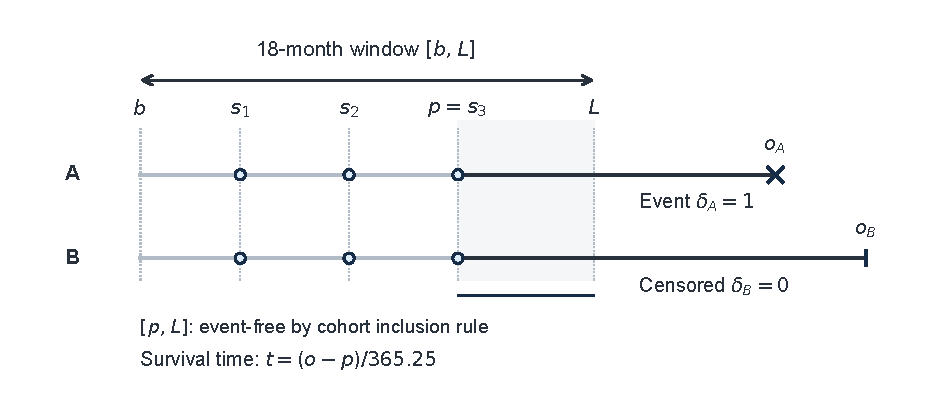
\includegraphics[width=\textwidth]{image_en/concept-survival.pdf}
\caption{Illustration of progression events and right-censoring in survival analysis}
\label{fig:concept-survival}
\end{figure}

The Cox proportional hazards model \cite{cox1972regression} expresses the instantaneous event rate (hazard function) $h_i(t)$ of individual $i$ at time $t$ as the product of two components:
\begin{equation}
 h_i(t)=h_0(t)\exp(\eta_i).
 \label{eq:cox-hazard}
\end{equation}
Here, $h_0(t)$ denotes the population-level \emph{baseline hazard function} over time, while $\eta_i = f_\theta(x_i)$ represents the individual \emph{log-risk score} estimated from input features $x_i$ via a deep neural network parameterized by $\theta$ (following the paradigm of DeepSurv \cite{katzman2018deepsurv}). A key advantage of the Cox formulation is that the hazard ratio between any two individuals $i$ and $j$ equals $\exp(\eta_i - \eta_j)$, which is entirely independent of time $t$. This implies that an individual assigned a higher log-risk score $\eta$ exhibits a higher instantaneous risk of progression at every point across the follow-up horizon.

By virtue of this time-invariance property, training the neural network does not require estimating the nonparametric baseline hazard $h_0(t)$; instead, one directly minimizes the negative Cox partial log-likelihood \cite{cox1972regression,katzman2018deepsurv}:
\begin{equation}
 \mathcal L_{\rm Cox}=-\sum_{i:\delta_i=1}\left[\eta_i-\log\sum_{j\in\mathcal R(t_i)}\exp(\eta_j)\right],
 \label{eq:cox-loss}
\end{equation}
where $\mathcal R(t_i)=\{j:t_j\geq t_i\}$ denotes the \emph{risk set} comprising all individuals who remain under active follow-up and have not experienced an event just prior to time $t_i$. Intuitively, this loss function compels the model to assign a higher risk score $\eta_i$ to the individual experiencing an event at $t_i$ than the scores $\eta_j$ of all individuals remaining event-free in the risk set at that moment; meanwhile, right-censored participants still contribute appropriately to the normalizing denominator $\mathcal R(t_i)$ up until the time they leave the study. When multiple events occur at tied survival times, I employ Breslow's approximation so that tied events share a common risk-set denominator consistently \cite{breslow1974covariance}. To evaluate the model's global ranking capability, the standard metric is Harrell's concordance index (C-index)---representing the proportion of comparable patient pairs in which the individual who experiences the event earlier is correctly assigned a higher risk score \cite{harrell1996multivariable}.

In longitudinal data analysis, a closely related methodological concept is \emph{landmarking}: at a pre-specified landmark time point, the prognostic model utilizes only information collected up to that landmark to predict future outcomes among individuals who remain event-free in the risk set \cite{vanhouwelingen2007dynamic}. The exact definition of the observation window and cohort eligibility milestone used in this thesis is detailed in Chapter~\ref{chap:method}.

\subsection{Time-Aware LSTM (T-LSTM) and Additive Attention}
\label{sec:background-temporal}
Long Short-Term Memory (LSTM) networks process sequential data effectively by maintaining and updating an internal memory state across successive steps \cite{hochreiter1997lstm}. However, standard LSTM architectures implicitly assume that the elapsed time between any two consecutive sequence steps is uniform. In real-world clinical records, the time gap between two consecutive visits varies substantially: it might be 3 months for one patient but up to 12 months for another. Clearly, clinical observations recorded 12 months ago generally carry less immediate relevance to the current state than observations acquired just 3 months prior \cite{baytas2017patient}.

The Time-Aware LSTM (T-LSTM) architecture proposed by Baytas et al. \cite{baytas2017patient} overcomes this limitation by incorporating the actual elapsed time interval $\Delta t$ between consecutive visits directly into the memory update equations: the previous cell memory $c_{t-1}$ is decomposed into a long-term component (preserved intact) and a short-term component (discounted monotonically as a decreasing function of $\Delta t$) before being combined with the new information from the current visit.

Once the T-LSTM generates the sequence of hidden states $h_t$ corresponding to each clinical visit, rather than passively relying only on the final hidden state, the model employs an additive attention mechanism to adaptively aggregate all visits using data-driven weights. The concept of weighted sequence aggregation originates from Bahdanau et al. \cite{bahdanau2015attention}; in this thesis, I implement scoring via a learnable context vector $\bm v$ following Yang et al. \cite{yang2016hierarchical}:
\begin{equation}
 e_t=\bm v^\top\tanh(W_hh_t+b_h),\qquad
 \alpha_t=\frac{\exp(e_t)}{\sum_k\exp(e_k)},\qquad
 z=\sum_t\alpha_th_t.
 \label{eq:additive-attention}
\end{equation}
Here, the attention weight $\alpha_t \in (0,1)$ quantifies the relative informational contribution of visit $t$, and $z$ serves as the unified longitudinal representation summarizing the patient's entire visit history. Figure~\ref{fig:concept-longitudinal} illustrates the synergistic integration of T-LSTM and additive attention across a three-visit sequence.

\begin{figure}[H]
\centering
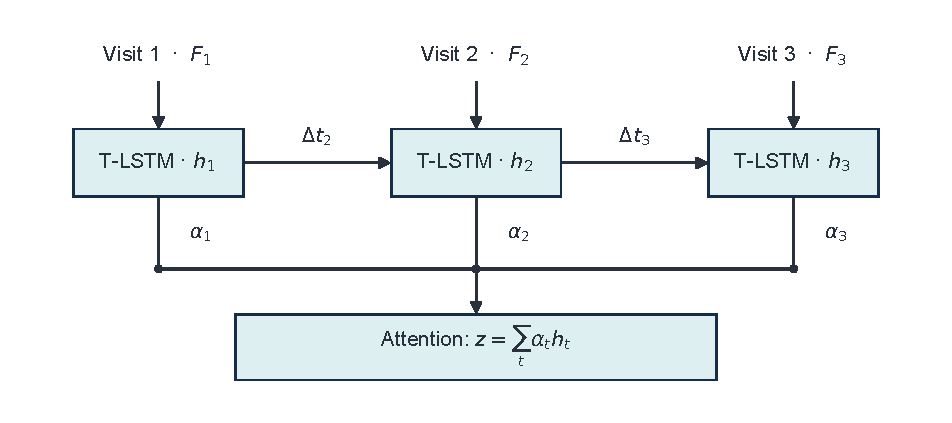
\includegraphics[width=\textwidth]{image_en/concept-longitudinal.pdf}
\caption{Principle of aggregating irregularly spaced longitudinal visit sequences via T-LSTM and additive attention}
\label{fig:concept-longitudinal}
\end{figure}

\section{The Three Information Sources and Feature Representations}
This thesis integrates three standard and widely adopted data modalities in Alzheimer's disease research: 3D structural MRI scans, whole-brain radiomics features, and clinical assessment scores. Table~\ref{tab:background-inputs} and Figure~\ref{fig:concept-sources} summarize the informational nature and specific technical considerations of each modality.

\begin{table}[H]
\centering\small
\caption[The three information sources in the prognostic task]{Informational nature and technical considerations of the three input modalities.}
\label{tab:background-inputs}
\begin{tabularx}{\linewidth}{@{}L{2.5cm}Y Y@{}}
\toprule
\textbf{Modality} & \textbf{Primary Information} & \textbf{Key Technical Consideration} \\
\midrule
3D structural MRI & Brain anatomical morphology; automated representation learning via 3D CNN & Requires standardizing head pose, voxel grid dimensions, and intensity scale without distorting anatomical geometry \\
Radiomics & Quantitative mathematical descriptors of shape, intensity distribution, and tissue texture & Texture feature values depend on the gray-level discretization scheme \cite{zwanenburg2020ibsi} \\
Clinical scores & Cognitive test (MMSE) and functional rating (CDR) scores & Directly tied to the outcome event definition; requires strict separation between input and outcome windows \\
\bottomrule
\end{tabularx}
\end{table}

\begin{figure}[H]
\centering
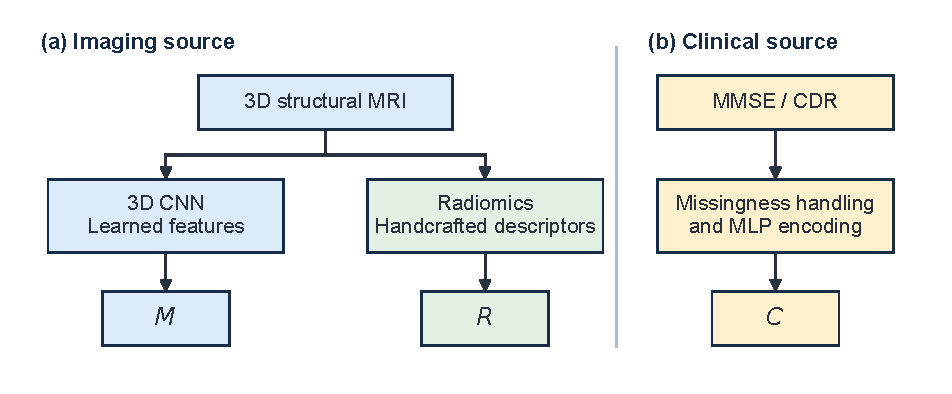
\includegraphics[width=\textwidth]{image_en/concept-sources.pdf}
\caption{Provenance and relationships among the three data representation streams at each visit}
\label{fig:concept-sources}
\end{figure}

More specifically, each information source fulfills a specialized representational role:
\begin{enumerate}
\item \emph{3D structural MRI}: visually captures brain anatomical morphology at the time of scanning \cite{jack2008adnimri}. In medical deep learning, 3D residual convolutional architectures such as ResNet \cite{he2016deep}, particularly when initialized with weights pretrained on diverse 3D medical imaging datasets such as MedicalNet \cite{chen2019med3d}, are widely favored for learning representations directly from the whole-brain volume---rather than cropping only the local hippocampal region as in several earlier studies \cite{li2019hippocampal}.
\item \emph{Radiomics features}: represent explicitly defined mathematical descriptors designed to quantify spatial geometry, first-order voxel intensity statistics, and spatial texture patterns within the brain mask (such as contrast derived from the Gray-Level Co-occurrence Matrix, GLCM). These feature definitions have been rigorously standardized by the IBSI community \cite{zwanenburg2020ibsi} and implemented in the PyRadiomics library \cite{vangriethuysen2017computational}. Because radiomics feature sets are typically high-dimensional and exhibit strong internal collinearity, Principal Component Analysis (PCA) \cite{jolliffe2016pca} serves as an effective dimensionality reduction tool prior to neural network encoding.
\item \emph{Clinical data}: the MMSE scale \cite{folstein1975mmse} evaluates global cognitive function, whereas the CDR scale \cite{morris1993cdr} assesses both cognitive performance and functional independence in daily life. Scores collected during the input observation window provide direct signals regarding the patient's current clinical state, kept strictly separate from post-milestone assessments used to determine progression outcomes.
\end{enumerate}

\section{Multimodal Fusion and Interaction Parameterization}
\label{sec:background-fusion}
Once each data modality has been mapped into a feature vector, the next central challenge is fusing them into a joint representational space \cite{baltrusaitis2019multimodal}. The most direct and common strategy is \emph{concatenation}: stacking the constituent vectors end to end to form a longer vector. While concatenation introduces no extra parameters at the combination step, its inherent limitation is that it fails to explicitly construct second-order cross-modal terms; consequently, discovering complex nonlinear relationships across modalities is left entirely to subsequent hidden layers.

In contrast, the \emph{outer product} multiplies every coordinate of the first modality by every coordinate of the second modality, explicitly constructing all second-order bilinear pairwise interactions \cite{zadeh2017tensor}. Figure~\ref{fig:concept-fusion} illustrates this fundamental distinction on two 2-dimensional vectors: concatenation yields a 4-element vector of independent coordinates, whereas the outer product forms a $2\times2$ matrix containing all four cross-products $x_i y_j$.

\begin{figure}[H]
\centering
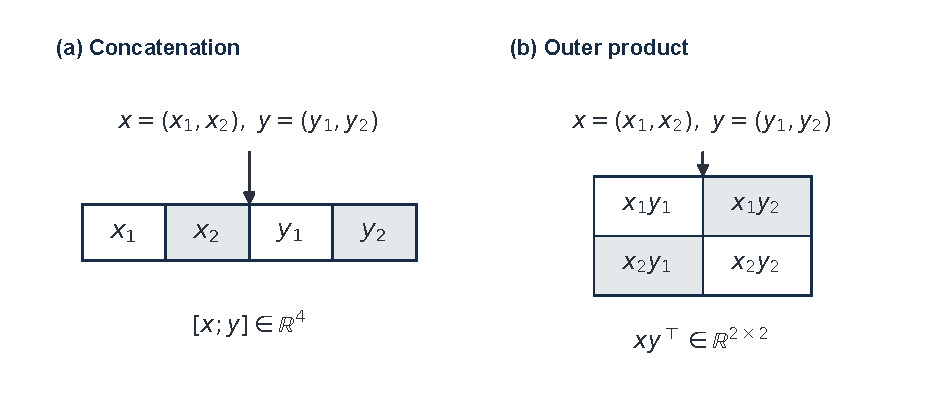
\includegraphics[width=\textwidth]{image_en/concept-fusion.pdf}
\caption{Comparison between feature concatenation and outer-product interaction on a two-dimensional example}
\label{fig:concept-fusion}
\end{figure}

\subsection{From Outer Products to Low-Rank CP Tensor Decomposition}
The primary obstacle to deploying full outer products in neural architectures is computational parameter explosion. Consider two arbitrary feature vectors $x\in\mathbb R^{d_x}$ and $y\in\mathbb R^{d_y}$. If the outer-product matrix $xy^\top \in \mathbb R^{d_x\times d_y}$ is flattened and projected through a standard linear layer into a $d_o$-dimensional output space, each output coordinate $h_k$ ($k=1,\dots,d_o$) is computed as a weighted combination of all cross-products:
\begin{equation}
 h_k=\sum_{i=1}^{d_x}\sum_{j=1}^{d_y}\mathcal W_{kij}x_i y_j+b_k,
 \label{eq:full-bilinear}
\end{equation}
where $\mathcal W\in\mathbb R^{d_o\times d_x\times d_y}$ acts as a third-order weight tensor. Under this formulation, the number of learnable weights reaches $d_o d_x d_y$ (excluding the bias vector $b$). For the actual dimensions used in this thesis ($d_x=32$, $d_y=32$, and $d_o=128$), a single bilinear interaction layer alone requires $32 \times 32 \times 128 = 131\,072$ weights---an excessively large capacity relative to a training cohort of a few hundred patients, placing the model at high risk of overfitting \cite{liu2018lowrank}.

To eliminate this parameter bottleneck while retaining the capacity to capture bilinear interactions, \emph{Canonical Polyadic (CP) tensor decomposition} \cite{carroll1970candecomp,kolda2009tensor} approximates the third-order weight tensor $\mathcal W$ as a sum of $Q$ rank-one tensors, where $Q$ is a small positive integer termed the \emph{decomposition rank}:
\begin{equation}
 \mathcal W_{kij}\approx\sum_{q=1}^Q O_{kq}A_{iq}B_{jq}.
 \label{eq:cp-concept-math}
\end{equation}
Substituting Eq.~(\ref{eq:cp-concept-math}) into Eq.~(\ref{eq:full-bilinear}) and rearranging the summation order reduces the cumbersome three-way tensor projection into a sequence of three lightweight operations:
\begin{equation}
 h=O\bigl[(A^\top x)\odot(B^\top y)\bigr]+b,
 \label{eq:cp-hadamard}
\end{equation}
where $A\in\mathbb R^{d_x\times Q}$, $B\in\mathbb R^{d_y\times Q}$, and $O\in\mathbb R^{d_o\times Q}$ are three low-rank factor matrices optimized directly via backpropagation, and $\odot$ denotes the element-wise Hadamard product. Rather than multiplying all coordinate pairs in the original space before compressing, the CP factorization projects $x$ and $y$ into a shared $Q$-dimensional latent space first, computes element-wise products within this low-rank space, and then projects the result linearly to the $d_o$-dimensional output space (Figure~\ref{fig:cp-intro}). Returning to the example with $d_x=32, d_y=32, d_o=128$: choosing rank $Q=8$ reduces the learnable weight count dramatically from $131\,072$ down to $Q(d_x + d_y + d_o) = 8 \times (32+32+128) = 1\,536$ (a reduction of nearly 99\%). This low-rank parameterization principle also forms the core foundation of prominent multimodal fusion architectures such as LMF \cite{liu2018lowrank} and MUTAN \cite{benyounes2017mutan}.

\begin{figure}[H]
\centering
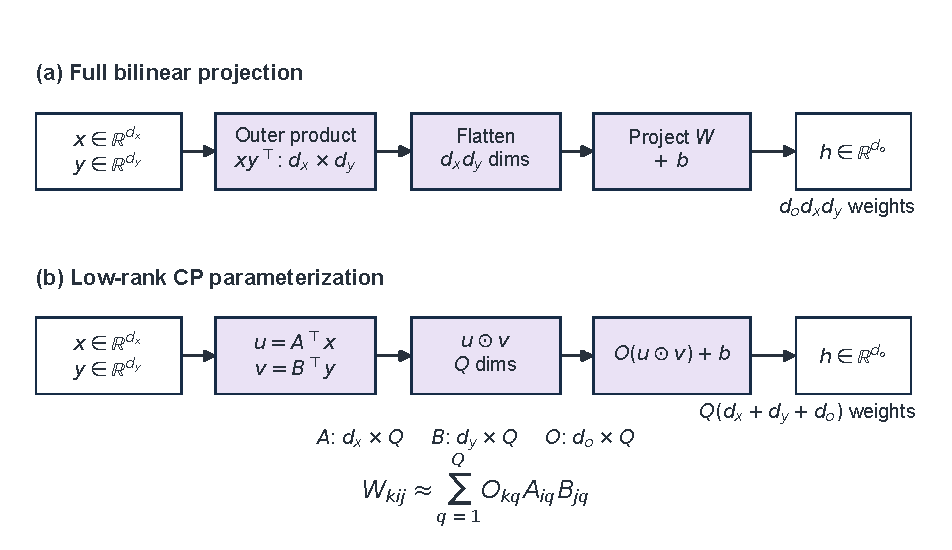
\includegraphics[width=\textwidth]{image_en/cp-concept-general.pdf}
\caption{Comparison between full bilinear projection and low-rank CP parameterization}
\label{fig:cp-intro}
\end{figure}

\subsection{Principle of Gated Residual Connections}
Once a bilinear interaction representation between two sources has been computed, completely replacing each modality's original representation with the interaction vector risks losing modality-specific signals, especially when one of the two sources suffers from measurement noise. To address this vulnerability, an effective principle in multimodal fusion is \emph{gated residual fusion}: preserving the direct pathway of the original representation and adding the interaction component only after modulating it through an input-dependent adaptive gate.

This principle has demonstrated effectiveness across diverse application domains; two recent arXiv preprints in multimodal video analysis illustrate representative variants:
\begin{enumerate}
\item \emph{Text Residual Fusion} by Ryumina et al. (2026) \cite{ryumina2026residual}: utilizes the text representation as the primary backbone stream, while audio, facial, and contextual streams contribute residual updates through input-dependent gates prior to layer normalization (Figure~\ref{fig:literature-gates}(a)).
\item \emph{DyFADet+} by Liu et al. (2026) \cite{liu2026motion}: treats the RGB visual stream as the main transmission pathway, while skeleton motion features pass through a gating unit scaled by a fixed constant $\alpha=0.5$ before residual addition (Figure~\ref{fig:literature-gates}(b)).
\end{enumerate}

\begin{figure}[H]
\centering
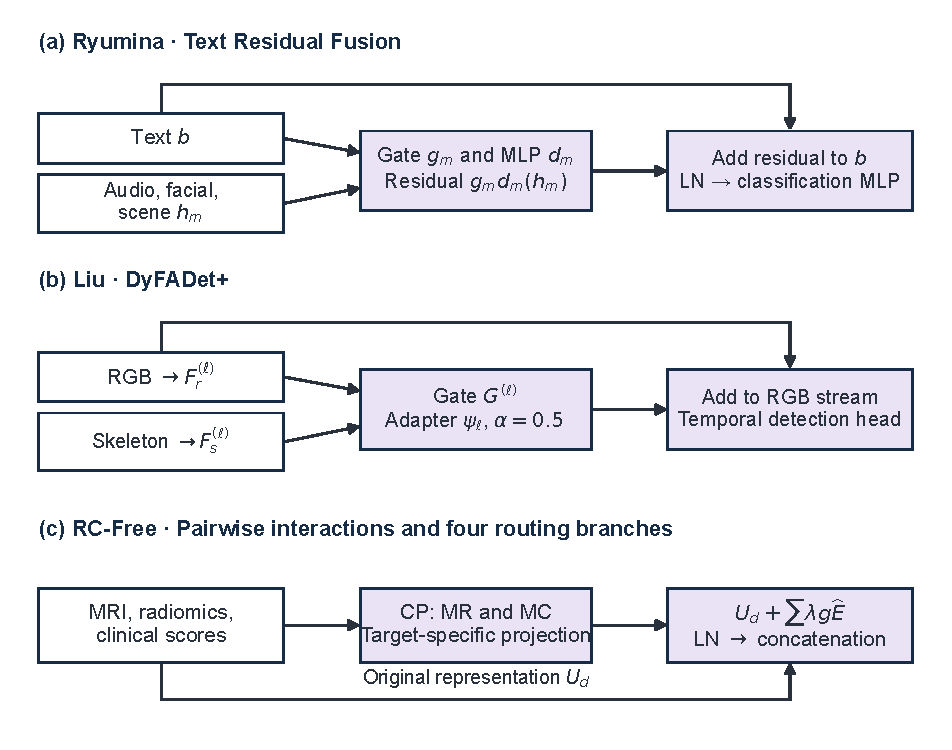
\includegraphics[width=\textwidth]{image_en/literature-gates.pdf}
\caption[Gated residual fusion mechanisms]{Illustration of gated residual connection principles synthesized by the author: (a) following Ryumina et al.~\cite{ryumina2026residual}, (b) following Liu et al.~\cite{liu2026motion}, and (c) the modality-specific gated residual routing scheme adopted in this thesis.}
\label{fig:literature-gates}
\end{figure}

Unlike the two aforementioned designs that anchor residual updates onto a single dominant stream, in the architecture proposed in this thesis, every input modality preserves its own dedicated representation pathway and receives pairwise interaction residuals through independent dynamic gates paired with learnable scaling coefficients (schematically illustrated in Figure~\ref{fig:literature-gates}(c)). The mathematical formulation and detailed architectural structure of this mechanism are presented in Section~\ref{sec:gated-routing} of Chapter~\ref{chap:method}.

\section{Related Work and Research Gaps}
\label{sec:related-work}
In recent years, numerous machine learning and deep learning methodologies have been proposed to tackle the problem of predicting MCI-to-dementia progression. Table~\ref{tab:related} systematizes four representative research directions in the literature and highlights the specific elements inherited by this thesis.

\begin{table}[H]
\centering\small
\renewcommand{\arraystretch}{1.02}
\caption[Summary of related work]{Major research directions, representative studies, and connections to this thesis.}
\label{tab:related}
\begin{tabularx}{\linewidth}{@{}L{2.8cm}Y Y@{}}
\toprule
\textbf{Approach} & \textbf{Representative Studies and Methods} & \textbf{Connection to This Thesis} \\
\midrule
Single-timepoint MRI & Li: hippocampal patches; Nakagawa: gray-matter volumes and deep survival network \cite{li2019hippocampal,nakagawa2020survival} & MRI representation learning within a survival analysis formulation \\
Longitudinal data & Li \& Fan: baseline MRI and longitudinal cognition \cite{li2019early}; Ding: cognitive and MRI sequences \cite{ding2023progression}; Dong: atrophy from longitudinal MRI pairs \cite{dong2021deepatrophy} & Exploiting temporal change dynamics for clinical prognosis \\
Radiomics and clinical scores & Tang et al.: LASSO--Cox combining radiomics, clinical scores, and laboratory markers \cite{tang2021individualized} & Motivation for verifying the complementary value of radiomics and clinical features \\
Longitudinal deep MRI survival & Aghajanian et al.: CNN--PCA--T-LSTM, attention, and Cox partial log-likelihood loss \cite{aghajanian2025longitudinal} & Direct reference pipeline, event definition, and risk stratification framework \\
\bottomrule
\end{tabularx}
\end{table}

Among these works, the study by Aghajanian et al. \cite{aghajanian2025longitudinal} serves as the most direct reference point. The authors selected 228 participants with MCI from ADNI who had at least three T1-weighted MRI scans within the first 18 months, employed a CNN to extract per-scan features, compressed them via PCA fitted on the training set (retaining 99\% explained variance), and trained a T-LSTM network (with an attention ablation) under the Cox loss. Crucially, when they experimented with concatenating gray-matter radiomics features into the T-LSTM with attention model, the discriminatory C-index decreased slightly rather than improving, leading the authors to retain only CNN-derived MRI features in their final model \cite{aghajanian2025longitudinal}.

\subsection{Research Gaps}
\label{sec:research-gaps}
It is important to emphasize that the negative conclusion regarding radiomics in Aghajanian et al. is tied to simple feature concatenation and a decoupled two-stage extraction pipeline. That result leaves open the question of whether explicitly modeling bilinear cross-modal interactions among MRI, radiomics, and clinical scores within a unified end-to-end deep learning architecture can unlock the prognostic potential of these complementary modalities. Motivated by this key research gap, I propose and empirically verify two architectural designs within a unified end-to-end training pipeline:
\begin{enumerate}[itemsep=0.1em,topsep=0.2em]
\item \emph{Parameterizing pairwise interactions via CP tensor decomposition}: replacing full bilinear projection layers with rank-$Q$ CP factorization to capture second-order cross-modal interactions while strictly controlling parameter complexity.
\item \emph{Pruning redundant direct interactions (RC-Free)}: retaining all three input modalities while activating only the two MRI-centered interaction pairs (MR and MC) and omitting the direct RC pair, then benchmarking this design systematically against all alternative pairwise topologies in Chapter~\ref{chap:results}.
\end{enumerate}

\chapter{Methodology}
\label{chap:method}

This chapter details the complete methodological framework and technical pipeline of this thesis following the exact data flow: beginning with a high-level architectural overview of the proposed RC-Free model (Section~\ref{sec:final-pipeline}); followed by cohort construction, curation, and dataset partitioning (Section~\ref{sec:study-design}); domain-specific preprocessing and encoding of the three input modalities (Section~\ref{sec:preprocessing}); the evolutionary progression of the multimodal fusion block from simple concatenation to the streamlined RC-Free topology (Section~\ref{sec:architecture-evolution}); irregular temporal sequence modeling trained under the Cox survival objective (Section~\ref{sec:temporal-method}); and finally, the multi-perspective survival evaluation framework (Section~\ref{sec:survival-evaluation}).

\section{Overview of the RC-Free Architecture}
\label{sec:final-pipeline}
The \textbf{RC-Free Pairwise Fusion (RC-Free)} architecture is designed for end-to-end training, mapping a three-visit multimodal sequence of an individual participant to a single scalar log-risk score $\eta_i \in \mathbb R$. Figure~\ref{fig:overall} outlines the four core processing stages of the model:
\begin{enumerate}
\item \emph{Modality-specific encoding}: At each clinical visit $t\in\{1,2,3\}$, the 3D MRI volume passes through a shared 3D ResNet-18 backbone to produce the anatomical representation $M_t\in\mathbb R^{128}$; PCA-compressed radiomics features pass through an MLP encoder to produce $R_t\in\mathbb R^{64}$; and standardized clinical scores concatenated with binary missingness indicators pass through an MLP encoder to produce $C_t\in\mathbb R^{64}$.
\item \emph{CP pairwise fusion and gated residual routing (RC-Free)}: The fusion module positions MRI as the central hub to compute two bilinear pairwise interactions---MRI--Radiomics (MR) and MRI--Clinical (MC)---via rank-$Q=8$ CP tensor decomposition. Four dynamically gated residual branches route these interaction signals back to enrich the original modality representations, yielding $(M_{\rm out}, R_{\rm out}, C_{\rm out})$; these updated vectors are subsequently concatenated (256 dimensions) and projected through $\operatorname{MLP}_{\rm out}$ into a unified visit representation $F_t\in\mathbb R^{128}$ for visit $t$.
\item \emph{Temporal sequence aggregation}: The visit sequence $(F_1, F_2, F_3)$ together with the actual elapsed time intervals between consecutive scans $(\Delta t_2, \Delta t_3)$ is processed by a T-LSTM network coupled with an additive attention mechanism to synthesize a single longitudinal representation $z\in\mathbb R^{128}$.
\item \emph{Survival risk estimation}: An output MLP head maps the longitudinal vector $z$ to a scalar log-risk score $\eta_i$, which is optimized directly under the Cox partial log-likelihood loss and evaluated using the C-index, Kaplan--Meier survival curves, and IPCW-AUC.
\end{enumerate}

\begin{figure}[H]
\centering
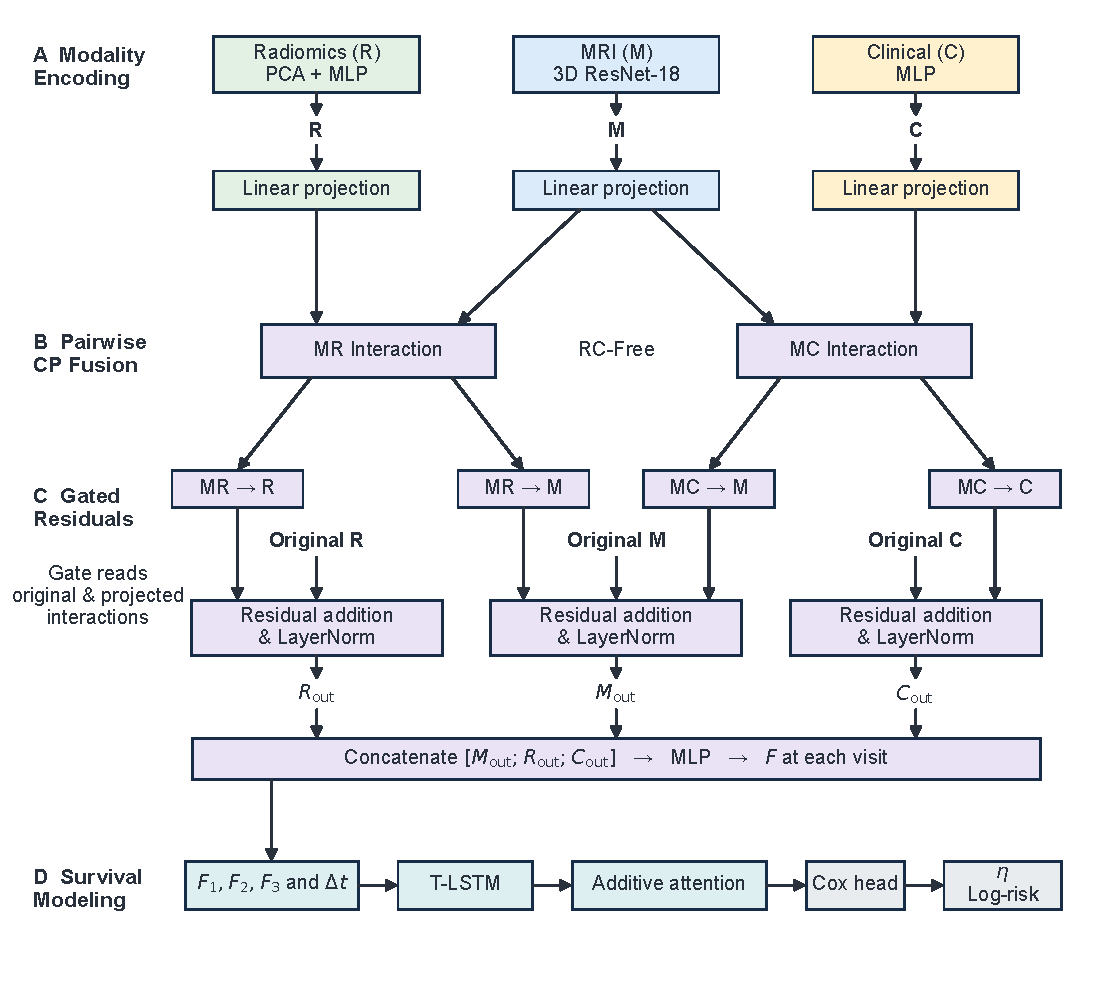
\includegraphics[width=\textwidth]{image_en/final-pipeline.pdf}
\caption{Overall processing pipeline of the proposed RC-Free model}
\label{fig:overall}
\end{figure}
\FloatBarrier

A comprehensive end-to-end schematic spanning raw data curation through survival evaluation is provided in Figure~\ref{fig:master-pipeline}, Appendix~\ref{app:master-pipeline}.

\section{Study Design and Cohort Construction}
\label{sec:study-design}

\subsection{Cohort Selection and the Three-Visit MRI Sequence}
All data analyzed in this study are extracted from the ADNI database \cite{weiner2015impact,jack2008adnimri} across three study phases: ADNI1, ADNIGO, and ADNI2. For each participant (uniquely identified by their Research Identifier, \texttt{RID}), I locate the earliest baseline visit coded as \texttt{bl} with a confirmed diagnosis of MCI (code 2 in the \texttt{DXSUM.DIAGNOSIS} field) \cite{adnidxsum}. Letting $b_i$ denote the baseline visit date, I define the \emph{cohort eligibility milestone} as $L_i = b_i + 18$ calendar months.

To ensure that all individuals enter the post-$L_i$ follow-up period prior to experiencing disease progression, a participant is excluded if they received a dementia diagnosis (code 3 in \texttt{DXSUM.DIAGNOSIS}) \cite{adnidxsum}, recorded an MMSE score $<24$, or had a CDR-global score $\geq 1$ at any time point at or before milestone $L_i$. In addition, each participant is required to have at least one valid cognitive follow-up assessment after $L_i$ to determine the clinical outcome.

Inheriting the three-scan-within-18-months longitudinal design of Aghajanian et al. \cite{aghajanian2025longitudinal}, I select three MRI scans within the observation window $[b_i, L_i]$ after clustering acquisitions separated by at least two months. When multiple scans exist within a single visit cluster, the selection rule prioritizes primary scans over repeat scans and ranks candidates according to ADNI's standardized preprocessing correction tags (prioritizing \texttt{GradWarp + B1 + N3 + Scaled} in ADNI1, and \texttt{GradWarp + N3m} in ADNIGO/ADNI2\footnote{Details on ADNI MRI preprocessing correction levels: \url{https://adni.loni.usc.edu/data-samples/adni-data/neuroimaging/mri/mri-pre-processing/}.}). If a participant has more than three valid scan clusters, the algorithm selects the first scan, the last scan, and the intermediate scan closest to the temporal midpoint, thereby guaranteeing the strict chronological ordering $s_{i1} < s_{i2} < s_{i3} \leq L_i$.

As illustrated in Figure~\ref{fig:cohort}, starting from 899 participants with successfully linked MRI identifiers, this filtering pipeline yields exactly \textbf{359 participants} with 1077 3D MRI volumes (comprising 78 participants from ADNI1, 80 from ADNIGO, and 201 from ADNI2), recording 106 progression events and 253 right-censored cases.

\begin{figure}[H]
\centering
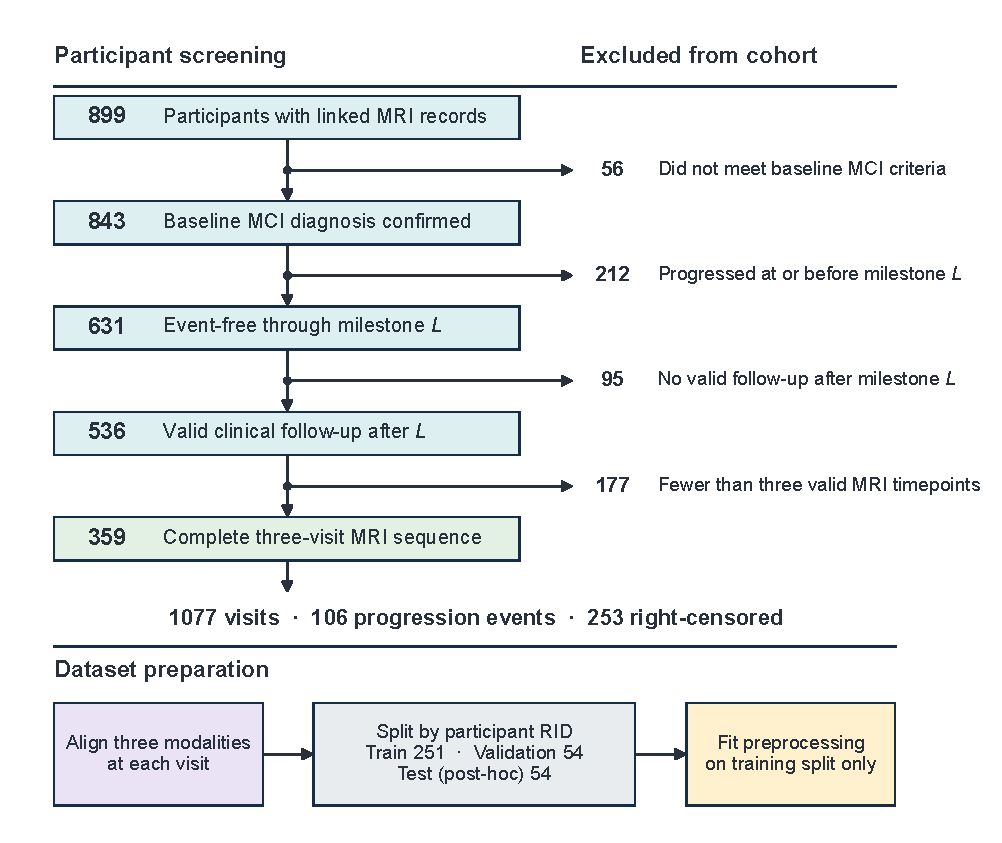
\includegraphics[width=\textwidth]{image_en/cohort-construction.pdf}
\caption{Workflow for longitudinal cohort construction and participant filtering}
\label{fig:cohort}
\end{figure}

\subsection{Outcome Events, Milestones, and Immortal Time Bias}
\label{sec:evaluation-scope}
Following the clinical criteria of Aghajanian et al. \cite{aghajanian2025longitudinal}, a progression event is recorded at the earliest valid clinical visit after milestone $L_i$ that satisfies either MMSE $<24$ or CDR-global $\geq 1$. If a participant never crosses these thresholds through the end of their available follow-up, they are treated as right-censored at their final valid clinical assessment. The survival time $t_i$ (measured in years) is computed from the third MRI scan date ($p_i = s_{i3}$) to the event or censoring date ($o_i$):
\begin{equation}
 t_i=\frac{o_i-p_i}{365.25},\qquad
 \delta_i=\begin{cases}1,&\text{if a progression event is recorded},\\0,&\text{if right-censored}.\end{cases}
 \label{eq:survival-target}
\end{equation}

When analyzing and interpreting Eq.~(\ref{eq:survival-target}), a critical methodological detail to note is the temporal offset between the third MRI scan date $p_i$ and the 18-month eligibility milestone $L_i$. Specifically, among the 359 participants in the cohort, 356 completed their third MRI scan prior to milestone $L_i$, with the gap $L_i - p_i$ having a median of 186 days (interquartile range: 169--197 days). Suppose a participant undergoes their third MRI scan at month 12 ($p_i$) while cohort eligibility is enforced up to month 18 ($L_i$): because the cohort filtering rules exclude all individuals who experienced cognitive decline at or before month 18, any participant retained in the dataset is guaranteed to be event-free between month 12 and month 18. In epidemiology and biostatistics, this guaranteed event-free interval from $p_i$ to $L_i$ is defined as ``immortal time''---a period during which study participants cannot experience the outcome event by design of the inclusion criteria. Including this interval in $t_i$ would induce \emph{immortal time bias} \cite{suissa2008immortal} if the model were interpreted as a prospective forecasting tool deployed immediately at scan date $p_i$. Consequently, all empirical results in this thesis are strictly interpreted for the retrospective risk-ranking task among participants known to have remained stable through milestone $L_i$.

Furthermore, the output $\eta_i$ of the Cox proportional hazards model represents a relative ranking score that orders progression risk across patients. Converting this relative score into an absolute probability of progression (expressed as a percentage at a specific time horizon) for an individual patient requires additionally estimating the baseline cumulative hazard function $H_0(t)$ \cite{cox1972regression}, a point discussed further in Chapter~\ref{chap:discussion}.

\subsection{Dataset Partitioning and Information Leakage Control}
\label{sec:data-split}
A common pitfall in longitudinal medical imaging is splitting individual scans rather than patients across training and evaluation sets; if two visits from the same participant appear in different splits, a model can memorize subject-specific brain anatomy rather than learning generalizable progression patterns. To completely prevent such subject-level leakage, the 359 eligible participants are partitioned strictly by participant identifier (\texttt{RID}) into three mutually exclusive cohorts:
\begin{itemize}[itemsep=0.2em,topsep=0.25em]
\item \emph{Training set} ($N=251$, 74 progression events, 29.5\%): used to optimize all network weights and fit every data-dependent preprocessing statistic.
\item \emph{Validation set} ($N=54$, 16 progression events, 29.6\%): used exclusively for early stopping, hyperparameter tuning, and selecting the final fusion topology.
\item \emph{Post-hoc test set} ($N=54$, 16 progression events, 29.6\%): held out in a locked state until all architectural choices and model checkpoints are finalized, providing an unbiased check of generalization.
\end{itemize}
Stratifying by outcome status preserves a nearly identical event rate (29.5--29.6\%) across all three splits, ensuring that validation and test evaluations reflect comparable censoring proportions.

Equally important is preventing \emph{preprocessing leakage}, which occurs when summary statistics from validation or test subjects influence how training features are scaled or imputed. In this pipeline, every tabular transformation---including the median values used to impute missing clinical scores, the per-feature means and standard deviations used for $z$-score standardization of radiomics and clinical variables, and the Principal Component Analysis (PCA) projection matrix applied to radiomics features---is fitted solely on the 251 training participants. Once fitted, these exact transformation parameters are frozen and applied unchanged to the validation and test sets. Furthermore, the input tensors fed to the model contain only baseline-window imaging, radiomics, and clinical predictors, with no diagnostic labels, event indicators ($\delta_i$), or follow-up durations ($t_i$).

To align multimodal records collected on slightly different clinic dates, each MRI scan is paired with the nearest valid MMSE and CDR assessment within a $\pm 90$-day matching window. Because the third MRI scan date $p_i$ can fall near the end of the 18-month observation window, this symmetric window means that 57 of the 359 participants have an MMSE or CDR score linked to their third MRI that was actually recorded after date $p_i$ (though still strictly prior to the outcome event or censoring date $o_i$). This retrospective matching detail is explicitly noted as a study limitation in Section~\ref{sec:study-limitations}.

Finally, Table~\ref{tab:baseline-characteristics} summarizes the baseline characteristics of all three splits at the first MRI scan, separated by stable ($\delta=0$) and progressing ($\delta=1$) participants. Across the training, validation, and test cohorts, participants have similar ages (mean $\approx 70$--$75$ years), education levels ($\approx 15$--$17$ years), baseline cognitive scores, and inter-visit scan intervals ($s_2-s_1 \approx 120$--$138$ days; $s_3-s_1 \approx 305$--$316$ days). Non-parametric Kruskal--Wallis and $\chi^2$ tests across the three splits all yield $p > 0.05$, confirming that the random participant-level partition produced well-balanced cohorts without systematic demographic or clinical bias.

\begin{landscape}
\begin{table}[p]
\centering\small
\caption[Participant characteristics at the first MRI]{Participant characteristics at the first MRI, stratified by dataset split and outcome status.}
\label{tab:baseline-characteristics}
\setlength{\tabcolsep}{2pt}
\begin{tabular}{@{}lrrrrrrr@{}}
\toprule
& \multicolumn{2}{c}{Training ($N=251$)} & \multicolumn{2}{c}{Validation ($N=54$)} & \multicolumn{2}{c}{Test ($N=54$)} & $p$ \\
\cmidrule(lr){2-3}\cmidrule(lr){4-5}\cmidrule(lr){6-7}
Characteristic & $\delta=0$ & $\delta=1$ & $\delta=0$ & $\delta=1$ & $\delta=0$ & $\delta=1$ & \\
\midrule
Participants & 177 & 74 & 38 & 16 & 38 & 16 & -- \\
Age at first MRI (years) & $71.64 \pm 7.5390$ & $73.41 \pm 7.1692$ & $71.29 \pm 8.6426$ & $74.86 \pm 5.6415$ & $70.03 \pm 7.5755$ & $72.74 \pm 6.7222$ & 0.4895 \\
Male, n (\%) & 96 (54.24) & 49 (66.22) & 23 (60.53) & 10 (62.50) & 28 (73.68) & 9 (56.25) & 0.3367 \\
Education (years) & $16.37 \pm 2.7171$ & $16.61 \pm 2.5846$ & $15.32 \pm 2.5691$ & $17.00 \pm 2.5298$ & $17.00 \pm 2.6304$ & $16.19 \pm 2.9489$ & 0.1465 \\
Baseline MMSE & $28.57 \pm 1.3799$ (53) & $27.22 \pm 1.7746$ (36) & $28.54 \pm 1.1266$ (13) & $27.75 \pm 1.4880$ (8) & $28.25 \pm 1.5275$ (16) & $26.83 \pm 2.0412$ (6) & 0.8688 \\
Baseline CDR-global & $0.44 \pm 0.1613$ (52) & $0.49 \pm 0.0833$ (36) & $0.38 \pm 0.2193$ (13) & $0.44 \pm 0.1768$ (8) & $0.47 \pm 0.1250$ (16) & $0.50 \pm 0.0000$ (6) & 0.2060 \\
Baseline CDR-SB & $0.92 \pm 0.5721$ (52) & $1.68 \pm 0.9573$ (36) & $1.04 \pm 0.8026$ (13) & $1.56 \pm 1.1476$ (8) & $1.28 \pm 0.9123$ (16) & $1.67 \pm 0.9309$ (6) & 0.7260 \\
$s_2-s_1$ (days) & $120.47 \pm 40.5683$ & $134.04 \pm 45.0152$ & $131.76 \pm 41.8372$ & $129.50 \pm 46.4672$ & $124.34 \pm 42.4470$ & $137.50 \pm 44.4627$ & 0.4313 \\
$s_3-s_1$ (days) & $305.12 \pm 44.1559$ & $313.04 \pm 42.8334$ & $307.32 \pm 34.0271$ & $312.19 \pm 75.3819$ & $312.08 \pm 55.0550$ & $315.50 \pm 38.4430$ & 0.8898 \\
$t_i$ (years), mean $\pm$ SD & $5.11 \pm 3.9055$ & $3.41 \pm 2.7858$ & $5.59 \pm 4.7319$ & $3.85 \pm 3.2066$ & $5.51 \pm 4.3420$ & $3.11 \pm 2.5391$ & 0.8713 \\
$t_i$ (years), median [Q1; Q3] & 3.64 [2.02; 7.54] & 2.09 [1.66; 4.42] & 3.92 [2.05; 6.73] & 3.69 [1.44; 4.88] & 4.06 [2.02; 8.20] & 2.42 [1.54; 3.64] & -- \\
\bottomrule
\end{tabular}
\par\vspace{6pt}
\begin{minipage}{0.96\linewidth}\small
$\delta=0$ denotes right-censoring and $\delta=1$ denotes an observed progression event. Unless otherwise noted, values are reported as sample mean $\pm$ SD. For MMSE and CDR, numbers in parentheses indicate the count of valid observations prior to median imputation. Male percentages are computed over participants with available sex records. Age is estimated from birth month and year by assuming the 15th day of the birth month. Demographic variables are taken from the nearest valid record up to the first MRI scan date. MMSE and CDR scores are matched within a $\pm90$-day window. The $p$-values assess differences across the three dataset splits (pooling both outcome statuses) using the Kruskal--Wallis test for continuous variables and the $\chi^2$ test for sex. $s_3-s_1$ denotes the elapsed time from the first to the third MRI scan, and $t_i$ denotes the survival time from the third MRI scan to event or censoring.
\end{minipage}
\end{table}
\end{landscape}


\section{Preprocessing and Modality Encoding}
\label{sec:preprocessing}
Figure~\ref{fig:input-three-sources} illustrates the three information sources linked at each clinical visit prior to entering their respective modality-specific encoders.

\begin{figure}[H]
\centering
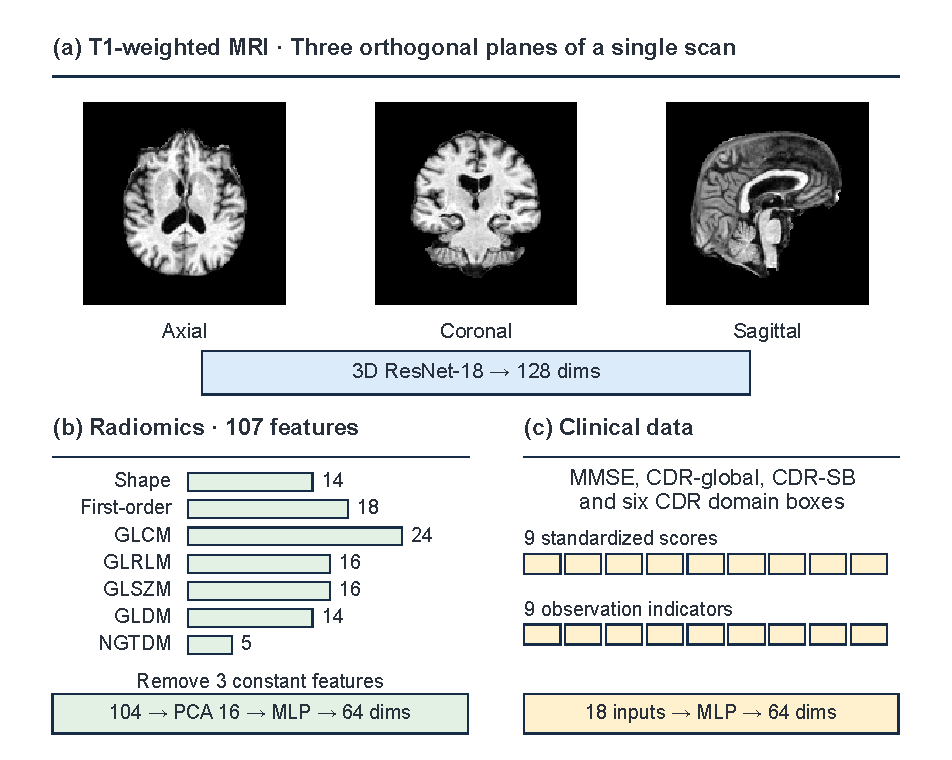
\includegraphics[width=\textwidth]{image_en/input-three-sources.pdf}
\caption[Three input modalities and feature representations]{The three input modalities and their feature representations.}
\label{fig:input-three-sources}
\caption*{\textit{Note.} The three orthogonal MRI planes are extracted by the author from a single preprocessed ADNI T1-weighted volume~\cite{jack2008adnimri}.}
\end{figure}

\subsection{3D MRI Branch and Shared Volumetric Encoder}
In longitudinal 3D brain MRI analysis, even a slight head tilt between consecutive scanning sessions causes the same anatomical structure (such as the hippocampus) to occupy different spatial coordinates, easily leading a neural network to confuse pose shifts with true pathological brain atrophy. Moreover, raw MRI voxel intensities are measured on an arbitrary relative scale that varies across scanners \cite{nyul1999standardizing}. Therefore, I establish a sequential preprocessing pipeline (Figure~\ref{fig:mri-preprocessing}) to standardize spatial orientation, voxel grid geometry, and intensity distribution without distorting the natural anatomical morphology of the brain:

\begin{figure}[H]
\centering
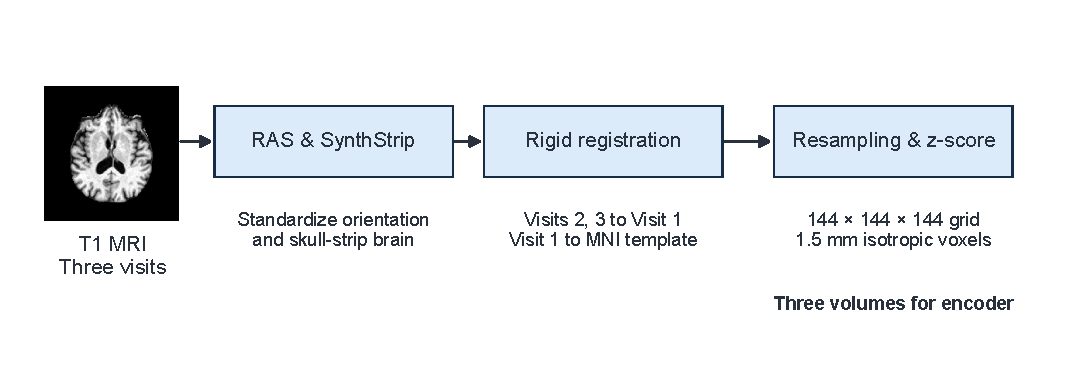
\includegraphics[width=\textwidth]{image_en/mri-preprocessing.pdf}
\caption{Preprocessing pipeline for longitudinal T1-weighted MRI sequences.}
\label{fig:mri-preprocessing}
\caption*{\textit{Note.} The diagram reuses an ADNI slice from Figure~\ref{fig:input-three-sources} to illustrate each step.}
\end{figure}

\begin{enumerate}
\item \emph{Axis reorientation and skull stripping}: All MRI volumes are reoriented to the standard anatomical RAS (\emph{Right--Anterior--Superior}) convention, after which the deep learning tool SynthStrip \cite{hoopes2022synthstrip} removes the skull and scalp tissues and generates a binary whole-brain mask (assigning 1 inside the brain parenchyma and 0 outside, without segmenting gray matter, white matter, or cerebrospinal fluid separately).
\item \emph{Intra-subject and MNI rigid registration}: For each participant, the second and third MRI scans are spatially aligned to that participant's first scan using a 6-degree-of-freedom \emph{rigid registration} (3 translations and 3 rotations, $\mathbf{x}'=\mathbf{R}\mathbf{x}+\mathbf{t}$). Subsequently, the first scan is rigidly aligned to the international standard template MNI152NLin2009cAsym \cite{mcgill2009icbm,fonov2009templates,fonov2011atlases} to establish a common anatomical coordinate frame across all subjects (Figure~\ref{fig:mri-registration}). This pipeline deliberately avoids affine scaling or nonlinear deformable warping so that true inter-subject brain size differences and longitudinal atrophy patterns are preserved intact.
\item \emph{Common grid resampling}: Both the intensity volume and the binary brain mask are resampled onto a uniform $144\times144\times144$ voxel grid with $1.5\text{ mm}$ isotropic resolution, using trilinear interpolation for intensity volumes and nearest-neighbor interpolation for masks to preserve exact binary $0/1$ labels.
\item \emph{Intra-mask intensity standardization}: For each scan independently, voxels inside the whole-brain mask undergo z-score normalization $z(v)=(I(v)-\mu)/\sigma$ (where $\mu$ and $\sigma$ are computed strictly over within-mask voxels of that individual scan) to center the intensity distribution at zero mean and unit variance, while voxels outside the mask are set to zero. No additional N4 bias-field correction is applied so as to preserve the native ADNI correction characteristics.
\end{enumerate}

\begin{figure}[H]
\centering
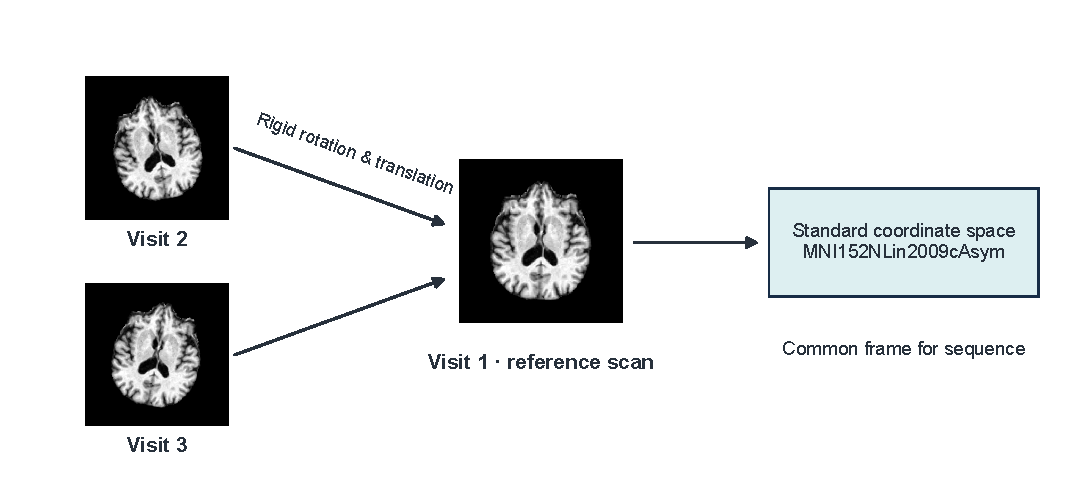
\includegraphics[width=\textwidth]{image_en/mri-registration.pdf}
\caption[Spatial registration across visits and MNI template]{Rigid spatial alignment across visits and to the MNI template.}
\label{fig:mri-registration}
\caption*{\textit{Note.} Poses are illustrated by rotating the same ADNI slice shown in Figure~\ref{fig:input-three-sources}.}
\end{figure}

Following preprocessing, all three MRI volumes of each participant pass through a shared \textbf{3D ResNet-18} encoder implemented in MONAI version 1.5.2\footnote{MONAI source code: \url{https://github.com/Project-MONAI/MONAI/blob/1.5.2/monai/networks/nets/resnet.py}.} \cite{he2016deep,cardoso2022monai}, initialized with complete convolutional weights and BatchNorm statistics pretrained on 3D medical imaging datasets from MedicalNet \cite{chen2019med3d} (with the original classification head removed) and fine-tuned end-to-end from the first training epoch. The backbone consists of four sequential 3D residual stages (with 64, 128, 256, and 512 channels, respectively) using BatchNorm \cite{ioffe2015batchnorm} and ReLU activations \cite{nair2010rectified}. After global average pooling produces a 512-dimensional vector, a linear projection layer ($512\to128$) followed by GELU \cite{hendrycks2016gelu}, Dropout 0.20 \cite{srivastava2014dropout}, and LayerNorm \cite{ba2016layernorm} produces the anatomical representation $M_t\in\mathbb R^{128}$ for each visit. Detailed intermediate feature map dimensions across all layers are listed in Table~\ref{tab:mri-encoder-shapes}, Appendix~\ref{app:mri-shapes}.

\subsection{Radiomics Feature Branch}
\label{sec:radiomics-pipeline}
In parallel with the abstract deep features learned by the 3D CNN, the radiomics branch extracts explicitly defined mathematical descriptors of whole-brain geometry and tissue texture directly from the MRI volume and binary brain mask using the PyRadiomics library \cite{vangriethuysen2017computational}. The extraction pipeline comprises four standardized steps:
\begin{enumerate}
\item \emph{Extraction of 107 features on the $[0,1]$ intensity scale}: Unlike the CNN branch which consumes z-score normalized volumes, the radiomics branch linearly rescales within-mask voxel intensities of each scan to the interval $[0,1]$ and discretizes gray levels using \texttt{binCount=64} \cite{pyradiomicsbins} prior to computing 107 features across 7 families: 3D shape (14 features), first-order intensity statistics (18 features), and five spatial texture matrix families---GLCM, GLRLM, GLSZM, GLDM, and NGTDM (75 features in total), summarized in Table~\ref{tab:radiomics-groups}.
\item \emph{Constant-feature removal}: Because within-mask intensities are rescaled to $[0,1]$, three first-order statistics (\texttt{Minimum}=0, \texttt{Maximum}=1, and \texttt{Range}=1) become constant across all scans and are removed, leaving 104 informative features.
\item \emph{Dimensionality reduction via PCA}: To mitigate severe multicollinearity among the 104 radiomics descriptors, I standardize each variable via z-score normalization and fit a PCA model \cite{jolliffe2016pca} exclusively on the training set with a threshold retaining at least 99\% of the total explained variance, yielding exactly 16 principal components per visit.
\item \emph{MLP encoding}: The 16-dimensional PCA vector passes through a two-layer MLP ($16\to128\to64$) equipped with GELU activation, Dropout 0.20, and LayerNorm to form the radiomics representation $R_t\in\mathbb R^{64}$.
\end{enumerate}

\begin{table}[H]
\centering\small
\caption{Seven radiomics feature families extracted from the 3D MRI volume.}
\label{tab:radiomics-groups}
\begin{tabularx}{\linewidth}{@{}L{2.7cm}r Y Y@{}}
\toprule
Family & Count & Descriptive information & Representative examples \\
\midrule
Shape & 14 & Geometric properties of the whole-brain mask & MeshVolume, SurfaceArea \\
First-order & 18 & Voxel intensity distribution within the mask & Mean, Variance, Entropy \\
GLCM & 24 & Gray-level co-occurrence relationships across voxel pairs & Contrast, Correlation \\
GLRLM & 16 & Run lengths of consecutive voxels sharing a gray level & ShortRunEmphasis, LongRunEmphasis \\
GLSZM & 16 & Sizes of connected homogeneous gray-level zones & SmallAreaEmphasis, LargeAreaEmphasis \\
GLDM & 14 & Gray-level dependency between a voxel and its neighborhood & DependenceEntropy, DependenceVariance \\
NGTDM & 5 & Intensity difference between a voxel and its neighbors & Coarseness, Contrast, Busyness, Complexity, Strength \\
\midrule
Total & 107 & 104 retained after removing Maximum, Minimum, and Range & PCA retains 16 components \\
\bottomrule
\end{tabularx}
\caption*{\textit{Note.} Definitions and representative features follow PyRadiomics~\cite{pyradiomicsfeatures}. Feature counts reflect the extraction catalog of this thesis.}
\end{table}


\subsection{Clinical Data Branch and Missingness Indicators}
The clinical branch leverages 9 prognostic variables (Table~\ref{tab:clinical-inputs}), comprising three composite scores (MMSE-total \cite{folstein1975mmse}, CDR-global, and CDR-SB) and six domain-specific CDR box scores \cite{morris1993cdr}. Any missing values are imputed using the training-set median of that variable at the corresponding visit index (falling back to the global training-set median if an entire visit column is missing), and subsequently standardized using the training-set mean and standard deviation.

Because an imputed value can numerically coincide with an observed clinical measurement, each clinical variable is paired with a \emph{binary observation indicator} (set to 1 if the measurement was actually observed, and 0 if it was missing prior to imputation), expanding the input vector from 9 to 18 dimensions (Figure~\ref{fig:clinical-18}). This 18-dimensional vector passes through a two-layer MLP ($18\to64\to64$) with GELU activation, Dropout 0.10, and LayerNorm to produce the clinical representation $C_t\in\mathbb R^{64}$.

\begin{table}[H]
\centering\small
\caption[Nine input clinical variables]{The nine pre-standardization clinical variables in the exact input order of the model. MMSE follows Folstein et al.~\cite{folstein1975mmse} and CDR follows Morris~\cite{morris1993cdr}. Each variable is paired with a corresponding binary observation indicator.}
\label{tab:clinical-inputs}
\begin{tabularx}{\linewidth}{@{}r L{3.6cm}Y@{}}
\toprule
Index & Clinical variable & Clinical meaning \\
\midrule
1 & MMSE-total & Global cognitive assessment total score, scale 0--30 \\
2 & CDR-global & Overall severity of cognitive and functional impairment \\
3 & CDR-SB & Sum of boxes across the six CDR domains, scale 0--18 \\
4 & CDR: Memory & Ability to retain and recall information \\
5 & CDR: Orientation & Awareness of time, place, and situational context \\
6 & CDR: Judgment & Judgment and problem-solving capability \\
7 & CDR: Community affairs & Independent participation in activities outside the home \\
8 & CDR: Home and hobbies & Ability to perform household tasks and maintain hobbies \\
9 & CDR: Personal care & Degree of independence in personal self-care \\
\bottomrule
\end{tabularx}
\end{table}


\begin{figure}[H]
\centering
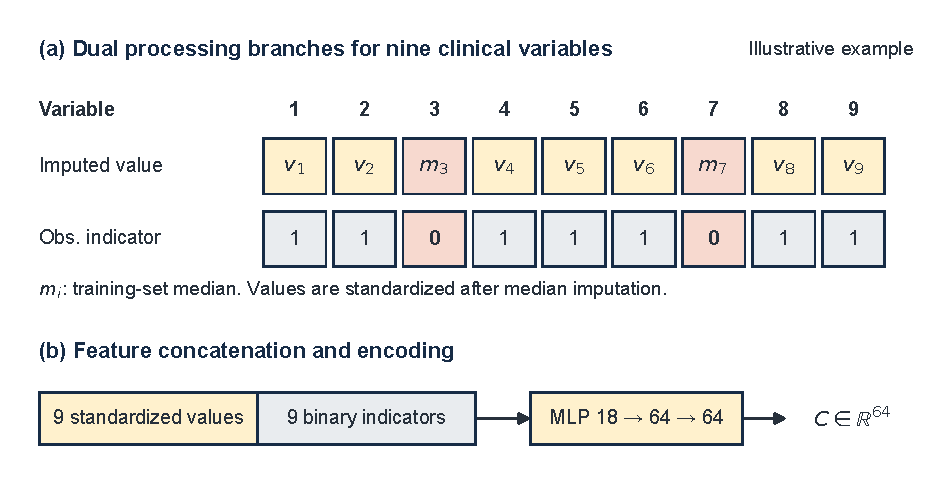
\includegraphics[width=\textwidth]{image_en/clinical-18-inputs.pdf}
\caption{Expanding nine clinical variables into an 18-dimensional input vector}
\label{fig:clinical-18}
\end{figure}

\section{Multimodal Fusion: From Concatenation to RC-Free}
\label{sec:architecture-evolution}
This section presents the systematic progression of the fusion module combining $(M_t, R_t, C_t)$ following the exact empirical verification sequence of this thesis: starting from unimodal MRI reference baselines (Section~\ref{sec:ref-models}), contrasting direct feature concatenation against pairwise outer-product interaction (Section~\ref{sec:pair-fusion}), compressing bilinear layers via CP tensor decomposition (Section~\ref{sec:cp-method}), and culminating in the dynamically gated residual routing mechanism and the streamlined RC-Free topology (Section~\ref{sec:gated-routing}).

\subsection{Reference Baselines on MRI Data}
\label{sec:ref-models}
To isolate the added value of longitudinal temporal dynamics and establish a rigorous benchmark against prior literature, this thesis constructs a sequence of unimodal MRI baselines (comprising a single-timepoint Last-MRI model, a 3-visit longitudinal MRI model with T-LSTM, and a longitudinal MRI model combining T-LSTM with additive attention) alongside an adapted re-implementation of the CNN--PCA--T-LSTM pipeline of Aghajanian et al. \cite{aghajanian2025longitudinal}. In this adapted re-implementation, a TensorFlow CNN processes $128^3$ MRI volumes and outputs 512-dimensional feature vectors; a PCA transform is fitted on the training set to retain 99\% variance (without feature scaling or whitening) before feeding a T-LSTM with a 64-dimensional hidden state. Table~\ref{tab:reference-methods} delineates the exact similarities and differences among the original published study, the adapted re-implementation, and the primary RC-Free model of this thesis. All primary models are implemented in PyTorch, MONAI, and scikit-learn \cite{paszke2019pytorch,cardoso2022monai,pedregosa2011sklearn}; differences in optimizer and batch size in the CNN--PCA--T-LSTM re-implementation are benchmarked on a unified basis via the validation C-index.

\begin{table}[H]
\centering\small
\caption[Comparison across the three methodologies]{Comparison of cohort data, configurations, and roles across methodologies.}
\label{tab:reference-methods}
\begin{tabularx}{\textwidth}{@{}L{3.2cm}Y Y@{}}
\toprule
\textbf{Methodology} & \textbf{Cohort and Preprocessing} & \textbf{Architecture and Role} \\
\midrule
Original Aghajanian \cite{aghajanian2025longitudinal} & 228 MCI subjects; SPM12, gray-matter volumes and gray-matter radiomics & CNN--PCA--T-LSTM; two-stage training; literature reference baseline \\
Adapted re-implementation & 359 subjects; MRI volumes resized to fixed $128^3$ grid & Per-seed CNN/PCA; 64-d T-LSTM; implementation benchmark \\
RC-Free Pairwise & 359 subjects; $144^3$ MRI, whole-brain radiomics, 18-d clinical input & MedicalNet; CP MR/MC; gated residuals; 128-d T-LSTM; primary proposed model \\
\bottomrule
\end{tabularx}
\end{table}

\subsection{Concatenation Baseline and Full Outer-Product Fusion}
\label{sec:pair-fusion}
When combining all three modality representations $(M_t\in\mathbb R^{128}, R_t\in\mathbb R^{64}, C_t\in\mathbb R^{64})$ simultaneously, the most direct baseline is \textbf{feature concatenation (Concatenation)}: keeping all three modality encoders unchanged, concatenating the three vectors directly into a 256-dimensional vector, and passing it through $\operatorname{MLP}_{\rm out}$ (a linear projection $256\to128$ followed by GELU, Dropout 0.20, and LayerNorm) to produce the visit representation $F_t\in\mathbb R^{128}$ for the temporal block (Figure~\ref{fig:concat-baseline}):
\begin{equation}
 F_t=\operatorname{MLP}_{\rm out}(M_t\concat R_t\concat C_t),\qquad
 M_t\concat R_t\concat C_t\in\mathbb R^{256},\quad F_t\in\mathbb R^{128}.
 \label{eq:concat}
\end{equation}

\begin{figure}[H]
\centering
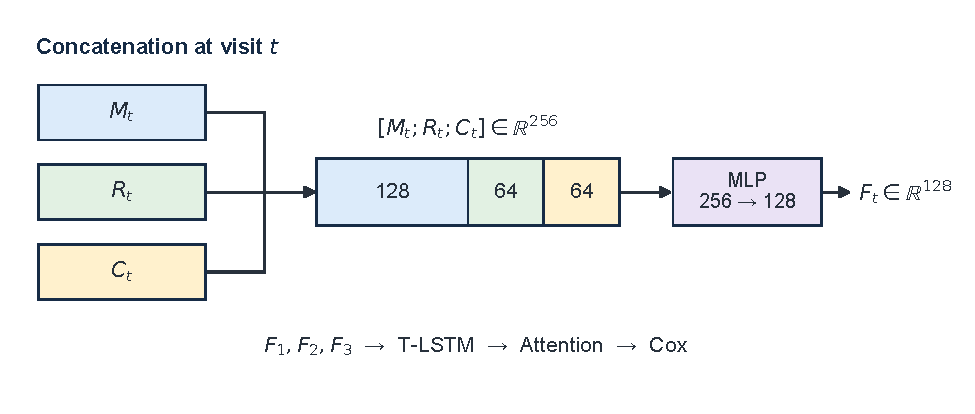
\includegraphics[width=\textwidth]{image_en/concat-baseline.pdf}
\caption[Three-modality concatenation baseline]{Computational flow of the three-modality concatenation baseline.}
\label{fig:concat-baseline}
\end{figure}

Under pure concatenation, discovering cross-modal relationships is left entirely to downstream projection layers. To overcome this limitation and explicitly capture bilinear interactions between modality pairs right before the concatenation step in Eq.~(\ref{eq:concat}), I construct the \textbf{Full Outer-Product} variant, which introduces three pairwise bilinear interaction modules: MR, MC, and RC. First, three bias-free linear projections reduce the dimensionality of each original modality representation to keep the outer-product space tractable:
\begin{equation}
 \widetilde M\in\mathbb R^{32},\qquad
 \widetilde R\in\mathbb R^{32},\qquad
 \widetilde C\in\mathbb R^{16}.
 \label{eq:input-projection}
\end{equation}

For each pair $k\in\{\mathrm{MR},\mathrm{MC},\mathrm{RC}\}$, let $x\in\mathbb R^{d_x}$ and $y\in\mathbb R^{d_y}$ denote the two dimension-reduced input vectors. The model computes the outer-product matrix $xy^\top \in \mathbb R^{d_x\times d_y}$, flattens it into a vector (1024 dimensions for MR; 512 dimensions for MC and RC), and passes it through a two-layer MLP equipped with GELU, Dropout 0.10, and LayerNorm (with layer dimensions MR: $1024\to128\to64$; MC: $512\to128\to64$; and RC: $512\to64\to32$), as illustrated in Figure~\ref{fig:mr-outer-product}. When all three pairwise modules are active, six routing branches project the resulting interaction representations back to the dimensionality of each constituent target modality to residually enrich the original representations prior to entering $\operatorname{MLP}_{\rm out}$ (Figure~\ref{fig:pair-update-routes}).

\begin{figure}[H]
\centering
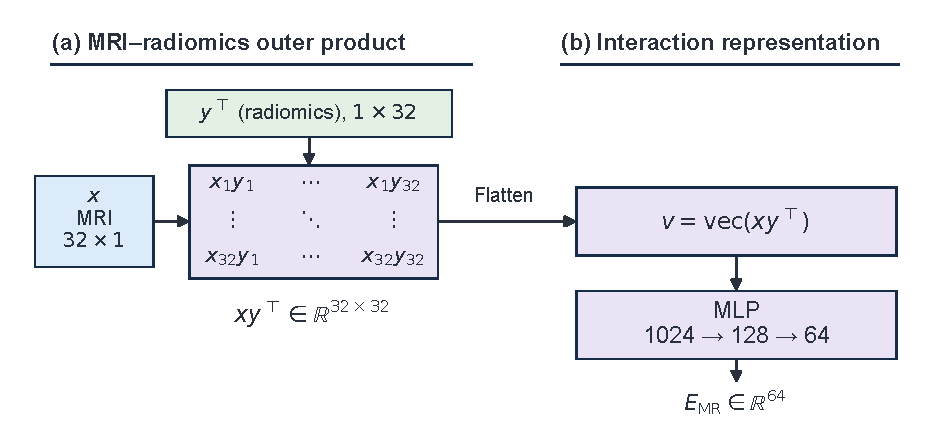
\includegraphics[width=\textwidth]{image_en/mr-outer-product.pdf}
\caption{Full outer-product and interaction MLP block (MR pair)}
\label{fig:mr-outer-product}
\end{figure}

\begin{figure}[H]
\centering
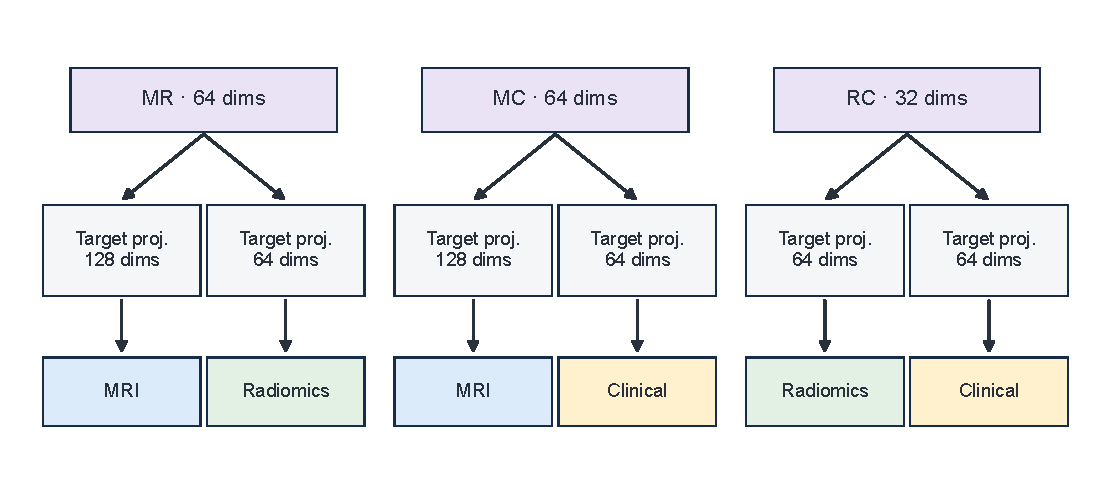
\includegraphics[width=\linewidth]{image_en/pair-update-routes.pdf}
\caption{Six update routing branches from three pairwise interactions}
\label{fig:pair-update-routes}
\end{figure}

\subsection{CP Tensor Parameter Compression}
\label{sec:cp-method}
As analyzed in Section~\ref{sec:background-fusion}, the initial linear projection layer immediately following an outer product corresponds to a third-order weight tensor $\mathcal W\in\mathbb R^{d_h\times d_x\times d_y}$ requiring $d_h d_x d_y + d_h$ parameters, which is highly prone to overfitting on a training cohort of 251 patients. To eliminate this bottleneck, I apply rank-$Q$ CP tensor decomposition according to Eqs.~(\ref{eq:cp-concept-math})--(\ref{eq:cp-hadamard}) \cite{carroll1970candecomp,kolda2009tensor,liu2018lowrank}: the initial bilinear layer of each interaction pair $k$ is replaced by three low-rank factor matrices $A\in\mathbb R^{d_x\times Q}$, $B\in\mathbb R^{d_y\times Q}$ (without bias), and $O\in\mathbb R^{d_h\times Q}$ (with bias vector $b$):
\begin{align}
 u&=A^\top x,\qquad v=B^\top y,\qquad q=u\odot v,\label{eq:cp-lowrank}\\
 h&=Oq+b,\qquad E_k=\operatorname{PostMLP}_k(h).
 \label{eq:cpblock}
\end{align}
Here, $\operatorname{PostMLP}_k$ retains the exact downstream architecture consisting of GELU activation, Dropout 0.10, a linear layer $d_h\to d_o$, and LayerNorm, outputting the pairwise interaction vector $E_k\in\mathbb R^{d_o}$ for pair $k\in\{\mathrm{MR},\mathrm{MC},\mathrm{RC}\}$ (specifically $E_{\mathrm{MR}}\in\mathbb R^{64}$, $E_{\mathrm{MC}}\in\mathbb R^{64}$, and $E_{\mathrm{RC}}\in\mathbb R^{32}$). This design guarantees a strictly fair experimental comparison: the CP variant modifies only the initial bilinear projection layer (Figure~\ref{fig:cp-block}) while keeping every subsequent layer identical to Full Outer-Product. The parameter count of the initial bilinear layer is thereby compressed from $d_h d_x d_y + d_h$ down to $Q(d_x+d_y+d_h)+d_h$. Table~\ref{tab:cpconfig} summarizes the dimensional configuration and CP rank for each pair (setting $Q=8$ for MR and MC, and $Q=4$ for RC due to its smaller output dimension).

\begin{figure}[H]
\centering
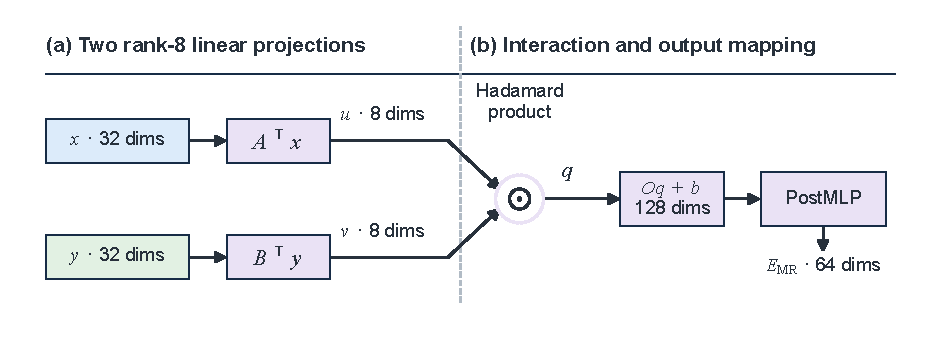
\includegraphics[width=\textwidth]{image_en/outer-vs-cp.pdf}
\caption{Rank-$Q=8$ CP interaction block for the MR pair}
\label{fig:cp-block}
\end{figure}

\begin{table}[H]
\centering\small
\caption{Dimensional configuration and CP rank across pairwise interaction modules}
\label{tab:cpconfig}
\begin{tabular}{lccccc}
\toprule
Pair & $(d_x,d_y)$ & Rank $Q$ & Hidden dim $d_h$ & Output dim $d_o$ & RC-Free \\
\midrule
MR & $(32,32)$ & 8 & 128 & 64 & Retained \\
MC & $(32,16)$ & 8 & 128 & 64 & Retained \\
RC & $(32,16)$ & 4 & 64 & 32 & Pruned \\
\bottomrule
\end{tabular}
\end{table}

\subsection{Gated Residual Routing and the Streamlined RC-Free Topology}
\label{sec:gated-routing}
\label{sec:rcfree-method}
Once the bilinear interaction representation $E_k\in\mathbb R^{d_o}$ has been extracted from each pair $k$ via Eq.~(\ref{eq:cpblock}), the next crucial step is routing this interaction information back to enrich the original representations of the two constituent modalities. Let $U_d$ denote the original representation of target modality $d\in\{M,R,C\}$ (i.e., $U_M=M\in\mathbb R^{128}$, $U_R=R\in\mathbb R^{64}$, and $U_C=C\in\mathbb R^{64}$). Because cross-modal interactions are not equally reliable across all patients or visits (for example, when an MRI scan suffers from motion artifacts or when clinical scores are imputed from missing entries), the proposed model does not add $E_k$ directly; instead, it routes the signal through a dynamically gated residual branch $k\to d$ comprising three sequential components (Figure~\ref{fig:route}):
\begin{enumerate}
\item \emph{Projecting $E_k$ into a target-aligned interaction vector $\widehat E_{k\to d}$}: The shared interaction vector $E_k$ cannot be added directly to the original representation $U_d$, first because of dimensional mismatch (for instance, $E_{\mathrm{MR}}$ has 64 dimensions whereas the target MRI representation $U_M$ has 128 dimensions), and second because the two constituent modalities in a pair need to extract distinct complementary cues from $E_k$. Therefore, on each routing branch $k\to d$, I apply a dedicated linear projection $W_{k\to d}$ (with bias $b_{k\to d}$ and no nonlinear activation) followed by LayerNorm to transform $E_k$ into a target-aligned interaction vector $\widehat E_{k\to d}$ matching the exact dimensionality of $U_d$:
\begin{equation}
 \widehat E_{k\to d}=\LN_{k\to d}(W_{k\to d}E_k+b_{k\to d}).
 \label{eq:target-projection}
\end{equation}
\item \emph{Sample-adaptive dynamic gate $g_{k\to d}\in(0,1)$}: The gating unit receives both the layer-normalized original representation and the target-aligned interaction vector simultaneously to determine a visit-specific opening weight through a 32-dimensional hidden MLP (initialized via Xavier uniform initialization \cite{glorot2010understanding} with zero initial biases) terminated by a sigmoid activation:
\begin{equation}
 g_{k\to d}=\sigma\!\left(
 w_{k\to d}^{\top}\operatorname{GELU}\!\left[
 V_{k\to d}\bigl(\LN_d^{\rm gate}(U_d)\concat\widehat E_{k\to d}\bigr)
 +a_{k\to d}\right]+c_{k\to d}\right).
 \label{eq:dynamic-gate}
\end{equation}
Using an independent sigmoid gate for each branch (rather than a softmax gate constrained to sum to 1) allows multiple branches to open concurrently when complementary signals are informative, or close toward 0 simultaneously when noise is detected.
\item \emph{Global scaling coefficient $\lambda_{k\to d}$}: A learnable scalar parameter shared across the dataset (initialized at $0.1$ without sign constraints) that modulates the overall amplitude and polarity of each routing branch.
\end{enumerate}

\begin{figure}[H]
\centering
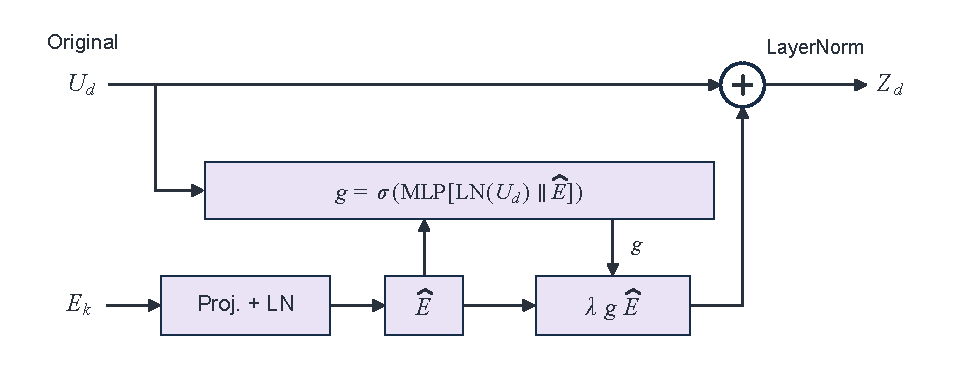
\includegraphics[width=\textwidth]{image_en/gated-residual-route.pdf}
\caption{Architecture of a single dynamically gated residual routing branch}
\label{fig:route}
\end{figure}

The updated representation of target modality $d$, after accumulating gated residuals from its set of active interaction pairs $\mathcal P(d)$, is normalized via a dedicated output LayerNorm:
\begin{equation}
 Z_d=\LN_d^{\rm out}\!\left(
 U_d+\sum_{k\in\mathcal P(d)}\lambda_{k\to d}\,g_{k\to d}\,\widehat E_{k\to d}
 \right).
 \label{eq:ours-residual}
\end{equation}
The three LayerNorm instances in Eqs.~(\ref{eq:target-projection})--(\ref{eq:ours-residual}) maintain completely independent parameter sets \cite{ba2016layernorm}. Whenever the dynamic gate $g_{k\to d}$ approaches 0, the interaction branch is effectively silenced and the output faithfully preserves the normalized original representation $\LN_d^{\rm out}(U_d)$.

The standard Full CP model maintains all three interaction pairs (MR, MC, and RC) along with all six residual routing branches. However, because radiomics features are mathematically extracted directly from the MRI volume itself, maintaining an additional direct interaction between radiomics and clinical scores (the RC pair) introduces potential representational redundancy once MRI is already directly coupled with both modalities. Motivated by this insight, I propose the streamlined \textbf{RC-Free} architecture: completely pruning the RC interaction module and positioning MRI as the central hub connecting the MR and MC pairs (both with decomposition rank $Q=8$), thereby reducing the number of gated residual routing branches from six to four while preserving all three input modalities (Figure~\ref{fig:rcfree-update}).

\begin{figure}[H]
\centering
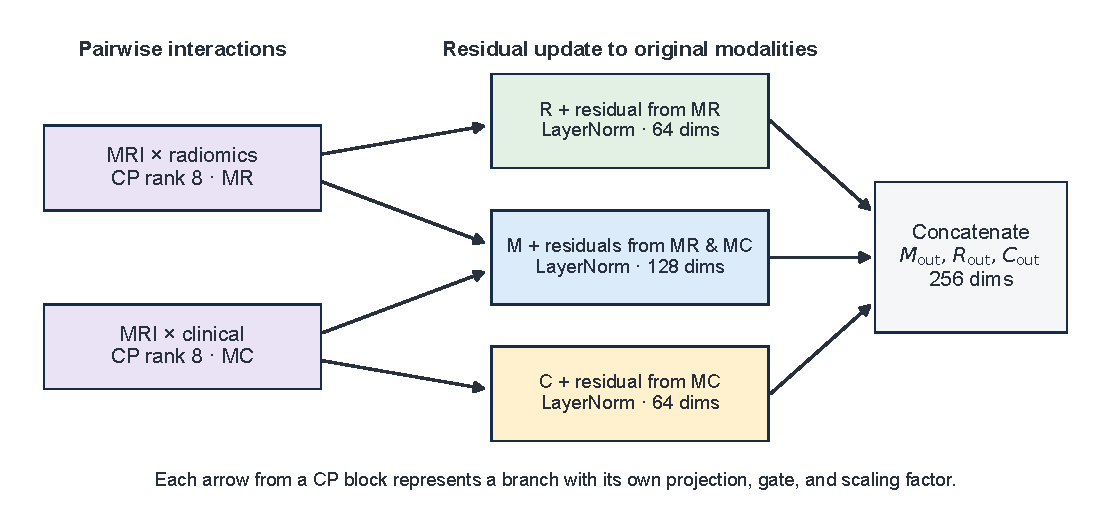
\includegraphics[width=\linewidth]{image_en/rcfree-update.pdf}
\caption{Four feature update routing branches in the proposed RC-Free architecture}
\label{fig:rcfree-update}
\end{figure}

Letting $D_{k\to d}=\lambda_{k\to d}\,g_{k\to d}\,\widehat E_{k\to d}$, the three updated modality representations in RC-Free take the explicit form:
\begin{align}
 M_{\rm out}&=\LN_M^{\rm out}(M+D_{(\mathrm{MR}\to M)}+D_{(\mathrm{MC}\to M)}),\label{eq:rcfree-first}\\
 R_{\rm out}&=\LN_R^{\rm out}(R+D_{(\mathrm{MR}\to R)}),\\
 C_{\rm out}&=\LN_C^{\rm out}(C+D_{(\mathrm{MC}\to C)}).
 \label{eq:rcfree-residual}
\end{align}
The three updated vectors $M_{\rm out}\in\mathbb R^{128}$, $R_{\rm out}\in\mathbb R^{64}$, and $C_{\rm out}\in\mathbb R^{64}$ are then concatenated into a 256-dimensional vector and projected through the same $\operatorname{MLP}_{\rm out}$ layer ($256\to128$, identical to Eq.~(\ref{eq:concat})) to obtain the fused visit representation $F_t\in\mathbb R^{128}$ at visit $t$. By keeping this 128-dimensional output interface fixed, varying the active set of pairwise interactions requires no changes to the downstream temporal modeling or survival prediction layers.

\section{Temporal Modeling and Cox Objective}
\label{sec:temporal-method}
\label{sec:training-method}
The sequence of three fused visit representations $F_t\in\mathbb R^{128}$ ($t=1,2,3$) together with the actual elapsed time intervals between consecutive scans $\Delta t_t=(s_t-s_{t-1})/365.25$ (measured in years, with $\Delta t_1=0$ by convention) is fed into a single-layer unidirectional temporal modeling block (Figure~\ref{fig:temporal}).

Adopting the T-LSTM formulation of Baytas et al. \cite{baytas2017patient} with a 128-dimensional hidden state, at time step $t$, the previous cell memory $c_{t-1}$ is decomposed into a short-term memory component $c_{t-1}^{S}$ (discounted by a monotonically decreasing decay weight $\gamma_t$ as $\Delta t_t$ increases) and a sustained long-term memory component $c_{t-1}^{L}$:
\begin{align}
 c_{t-1}^{S}&=\tanh(W_Sc_{t-1}+b_S),\qquad
 c_{t-1}^{L}=c_{t-1}-c_{t-1}^{S},\label{eq:tlstm-first}\\
 \gamma_t&=\frac{1}{\log(e+\Delta t_t)},\qquad
 c_{t-1}^{*}=c_{t-1}^{L}+\gamma_t c_{t-1}^{S}.
 \label{eq:tlstm-memory}
\end{align}
The time-adjusted memory state $c_{t-1}^{*}$ then enters the standard LSTM forget gate $f_t$, input gate $i_t$, output gate $o_t$, and candidate memory $\widetilde c_t$ equations (computed from $F_t$ and $h_{t-1}$):
\begin{equation}
 c_t=f_t\odot c_{t-1}^{*}+i_t\odot\widetilde c_t,
 \qquad h_t=o_t\odot\tanh(c_t).
 \label{eq:tlstm-state}
\end{equation}
(If a visit were flagged as invalid, the recurrent cell would carry forward its previous state; in our curated cohort, all three visits of every participant are valid.)

\begin{figure}[H]
\centering
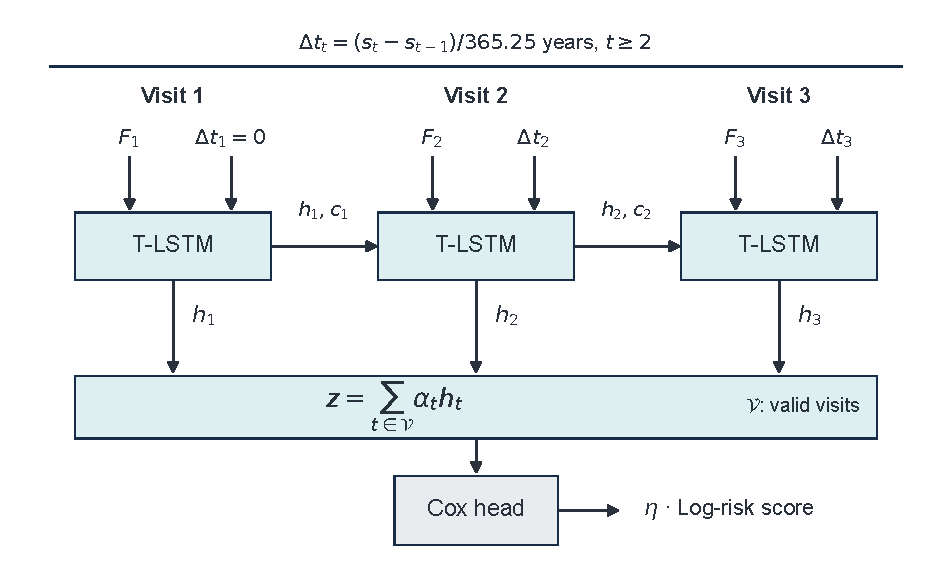
\includegraphics[width=\textwidth]{image_en/temporal-model.pdf}
\caption{Temporal T-LSTM block, additive attention, and Cox head}
\label{fig:temporal}
\end{figure}

Next, an additive attention mechanism (Eq.~(\ref{eq:additive-attention}) following Yang et al. \cite{yang2016hierarchical}) applies a $128\to64\to1$ scoring network to assign normalized importance weights $\alpha_t$ across the set of valid visits $\mathcal V$:
\begin{equation}
 e_t=v_a^\top\tanh(W_a h_t+b_a),\qquad
 \alpha_t=\frac{\exp(e_t)}{\sum_{j\in\mathcal V}\exp(e_j)},\qquad
 z=\sum_{t\in\mathcal V}\alpha_t h_t.
 \label{eq:temporal-attention}
\end{equation}
From the aggregated longitudinal representation $z\in\mathbb R^{128}$, an output MLP head ($128\to64$ with GELU activation and Dropout 0.30, followed by a linear layer $64\to1$) estimates the scalar log-risk score $\eta_i\in\mathbb R$ in the Cox proportional hazards model of Eq.~(\ref{eq:cox-hazard}). The entire network is trained end-to-end by minimizing the negative Cox partial log-likelihood (Eq.~(\ref{eq:cox-loss})) averaged over the $N_e$ observed events in a batch, handling tied event times via Breslow's approximation \cite{breslow1974covariance}:
\begin{equation}
 \mathcal L_{\rm Cox}=-\frac{1}{N_e}\sum_k
 \left[\sum_{i\in\mathcal D_k}\eta_i
 -d_k\log\!\left(\sum_{j\in\mathcal R_k}\exp(\eta_j)\right)\right],
 \label{eq:cox-method}
\end{equation}
where $\mathcal D_k$ denotes the set of individuals experiencing an event at distinct event time $\tau_k$ ($d_k=|\mathcal D_k|$) and $\mathcal R_k=\{j:t_j\geq\tau_k\}$ is the risk set at time $\tau_k$. The complete forward pass of the proposed RC-Free model is summarized in Algorithm~\ref{alg:rcfree-forward}.

\begin{algorithm}[H]
\caption{Forward pass of the RC-Free Pairwise Fusion model}
\label{alg:rcfree-forward}
\small
\textbf{Input:} A longitudinal sequence of three visits $(t=1,2,3)$ for an individual, consisting of preprocessed 3D MRI volumes, PCA-compressed radiomics feature vectors (16 dimensions), clinical vectors comprising nine standardized scores and nine observation indicators (18 dimensions), and elapsed inter-visit intervals $\Delta t_t$ (with $\Delta t_1=0$).\\
\textbf{Output:} Individual log-risk score $\eta\in\mathbb R$.
\begin{enumerate}[leftmargin=1.2em,label=\arabic*.,itemsep=0.2em]
\item For each visit $t=1,2,3$:
\begin{enumerate}[leftmargin=1.2em,label=\alph*.,itemsep=0.15em]
\item Encode the three input sources at visit $t$ into $M_t\in\mathbb R^{128}$, $R_t\in\mathbb R^{64}$, and $C_t\in\mathbb R^{64}$ as detailed in Section~\ref{sec:preprocessing}; apply bias-free linear projections to obtain reduced representations $\widetilde M_t\in\mathbb R^{32}$, $\widetilde R_t\in\mathbb R^{32}$, and $\widetilde C_t\in\mathbb R^{16}$ via Eq.~(\ref{eq:input-projection}).
\item Compute pairwise interaction representations $E_{\mathrm{MR},t}\in\mathbb R^{64}$ from $(\widetilde M_t,\widetilde R_t)$ and $E_{\mathrm{MC},t}\in\mathbb R^{64}$ from $(\widetilde M_t,\widetilde C_t)$ using two rank-$Q=8$ CP interaction blocks followed by their respective MLPs according to Eqs.~(\ref{eq:cp-lowrank})--(\ref{eq:cpblock}).
\item For each active routing branch $k\to d\in\{\mathrm{MR}\to M,\mathrm{MR}\to R,\mathrm{MC}\to M,\mathrm{MC}\to C\}$, compute the target-aligned projection $\widehat E_{k\to d,t}$ via Eq.~(\ref{eq:target-projection}), the dynamic gating coefficient $g_{k\to d,t}$ via Eq.~(\ref{eq:dynamic-gate}), and the gated residual update $D_{k\to d,t}=\lambda_{k\to d}\,g_{k\to d,t}\,\widehat E_{k\to d,t}$.
\item Apply residual updates and layer normalization according to Eqs.~(\ref{eq:rcfree-first})--(\ref{eq:rcfree-residual}) to obtain $M_{\mathrm{out},t}\in\mathbb R^{128}$, $R_{\mathrm{out},t}\in\mathbb R^{64}$, and $C_{\mathrm{out},t}\in\mathbb R^{64}$.
\item Concatenate the updated modality vectors and project them into the fused visit representation: $F_t=\operatorname{MLP}_{\mathrm{out}}(M_{\mathrm{out},t}\concat R_{\mathrm{out},t}\concat C_{\mathrm{out},t})\in\mathbb R^{128}$ via Eq.~(\ref{eq:concat}).
\end{enumerate}
\item Initialize hidden and cell states to zero; pass the temporal sequence $(F_t,\Delta t_t)_{t=1}^3$ through the T-LSTM cell according to Eqs.~(\ref{eq:tlstm-first})--(\ref{eq:tlstm-state}) to obtain hidden states $h_1,h_2,h_3\in\mathbb R^{128}$.
\item Compute additive attention weights $\alpha_t$ and the aggregated longitudinal representation $z=\sum_{t=1}^3\alpha_t h_t\in\mathbb R^{128}$ via Eq.~(\ref{eq:temporal-attention}).
\item Pass $z$ through the Cox survival prediction MLP head ($128\to64\to1$) described in Section~\ref{sec:training-method} to output the scalar log-risk score $\eta$.
\end{enumerate}
\end{algorithm}


\section{Risk Ranking and Survival Stratification Evaluation}
\label{sec:survival-evaluation}
A prognostic survival model must be evaluated simultaneously across three complementary dimensions (Figure~\ref{fig:evaluation-map}): global ranking concordance (C-index), longitudinal risk-group stratification (Kaplan--Meier curves), and time-horizon-specific discrimination (IPCW-AUC). All evaluations are computed on the out-of-sample risk scores $\eta_i$ generated by the three frozen RC-Free checkpoints (corresponding to the three random initializations).

\begin{figure}[H]
\centering
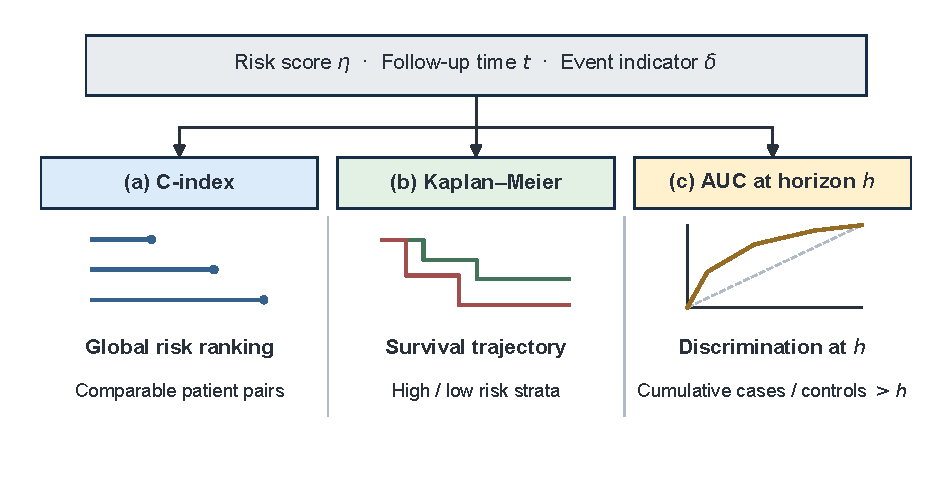
\includegraphics[width=\textwidth]{image_en/evaluation-map.pdf}
\caption{Three evaluation perspectives for survival risk ranking and stratification}
\label{fig:evaluation-map}
\end{figure}

\subsection{Harrell's Concordance Index (C-index)}
Harrell's C-index \cite{harrell1996multivariable} measures the proportion of comparable participant pairs ($t_i<t_j$ with $\delta_i=1$) in which the model correctly assigns a higher risk score to the individual who experiences the progression event earlier ($\eta_i>\eta_j$). A value of 0.5 corresponds to random guessing and 1.0 indicates perfect concordance. The validation set contains 480 comparable pairs and the post-hoc test set contains 528 comparable pairs; results are reported as sample mean $\pm$ standard deviation (SD) across the three random initializations.

\subsection{Kaplan--Meier Stratification via Consensus Risk Groups}
To verify whether the continuous risk score $\eta_i$ can separate patients into clinically distinct progression trajectories, I use the \emph{training-set median risk score} as a fixed cutoff threshold (strictly avoiding any threshold optimization on the validation or test sets): individuals scoring above the threshold are assigned to the high-risk group, and those at or below the threshold are assigned to the low-risk group. To reduce sensitivity to any single random initialization, the final group assignment for each participant is determined by \emph{majority-vote consensus} across the three seeds (assigning a participant to the high-risk group if at least 2 out of 3 seeds classify them as high-risk).

Given the resulting high- and low-risk groups, Kaplan--Meier survival curves \cite{kaplan1958nonparametric} estimate the probability of remaining event-free over time, plotted with 95\% confidence intervals, right-censoring ticks, and numbers at risk at 0, 2, 3, and 5 years. Separation between the two survival curves is tested via the nonparametric log-rank test \cite{mantel1966survival}, while a univariate Cox regression model estimates the hazard ratio (HR) and its 95\% confidence interval across the entire follow-up duration. The proportional hazards (PH) assumption is verified using scaled Schoenfeld residuals following Grambsch and Therneau \cite{grambsch1994proportional} (with rank-transformed time).

\subsection{IPCW Time-Dependent AUC at 2, 3, and 5 Years}
At each clinical evaluation horizon $h \in \{2, 3, 5\text{ years}\}$, I evaluate the model's ability to discriminate between cumulative cases up to horizon $h$ ($\mathcal C_h=\{i:\delta_i=1,t_i\leq h\}$) and dynamic controls who remain event-free beyond $h$ ($\mathcal D_h=\{j:t_j>h\}$) using the cumulative/dynamic AUC estimator \cite{hung2010time}. Because participants right-censored prior to $h$ have unknown event status at horizon $h$, naively omitting them would introduce censoring bias; therefore, each event case is weighted by the inverse probability of censoring $w_i = 1/\widehat G(t_i)$ (IPCW) \cite{polsterl2020scikit,hung2010time}, where the censoring survival distribution $\widehat G(\cdot)$ is estimated via the Kaplan--Meier method on the training set under the assumption of independent censoring \cite{sksurvauc}:
\begin{equation}
 \widehat{\operatorname{AUC}}(h)=
 \frac{\displaystyle\sum_{i\in\mathcal C_h}w_i
 \sum_{j\in\mathcal D_h}\kappa(\eta_i,\eta_j)}
 {\displaystyle |\mathcal D_h|\sum_{i\in\mathcal C_h}w_i},
 \qquad
 \kappa(a,b)=\begin{cases}
 1,&a>b,\\
 \tfrac12,&a=b,\\
 0,&a<b.
 \end{cases}
 \label{eq:ipcw-auc}
\end{equation}
Following the standard implementation in \texttt{scikit-survival}, two risk scores differing by no more than $10^{-8}$ are treated as tied \cite{sksurvauc}. To avoid extrapolating the training censoring distribution when the maximum follow-up time in the validation set (18.26 years) exceeds that of the training set (13.95 years), evaluation times are capped at $h+\varepsilon$ (determined via \texttt{nextafter}).

\chapter{Experiments and Results}
\label{chap:results}

This chapter presents a comprehensive empirical evaluation designed to verify each architectural hypothesis formulated in Chapter~\ref{chap:method}, strictly following the sequence of five research questions (RQ1--RQ5) established in Table~\ref{tab:rq}. To ensure scientific transparency and rigor, the experiments progress systematically from simple baselines to the complete proposed model: (1) evaluating the prognostic contribution of longitudinal temporal sequences and multimodal data integration (RQ1--RQ2); (2) testing the advantage of pairwise bilinear interactions over standard feature concatenation (RQ3); (3) quantifying the parameter compression achieved by CP decomposition and validating the streamlined RC-Free topology against all seven pairwise interaction combinations as well as the literature reference pipeline (RQ4--RQ5); and (4) verifying the practical survival stratification capability of RC-Free via time-dependent IPCW-AUC and Kaplan--Meier survival curves.

\section{Training Protocol and Convergence Dynamics}
\label{sec:experimental-protocol}
All experiments in this thesis utilize the fixed participant-level dataset partition detailed in Section~\ref{sec:data-split} (comprising 251 training, 54 validation, and 54 post-hoc test participants, corresponding to 74, 16, and 16 progression events, respectively), with all preprocessing parameters fitted exclusively on the training set. The validation set contains 480 comparable patient pairs and the post-hoc test set contains 528 comparable pairs. The initial exploratory input ablations (RQ1--RQ2) are conducted using a single random initialization; all core architectural comparisons and survival evaluations are repeated across three independent random seeds (20260727, 20260728, and 20260729), with metrics reported as sample mean $\pm$ standard deviation (SD).

Because 3D volumetric MRI sequences consume substantial GPU memory whereas the Cox partial log-likelihood objective is sensitive to small batch sizes, the training protocol is carefully configured as follows:
\begin{enumerate}
\item \emph{Optimization algorithm}: The model is optimized using AdamW \cite{loshchilov2019adamw} with an initial learning rate of $10^{-4}$, weight decay of $10^{-4}$, momentum parameters $(\beta_1,\beta_2)=(0.9,0.999)$, and gradient norm clipping at a threshold of $1.0$ \cite{pascanu2013difficulty} to ensure training stability.
\item \emph{Batch size, gradient accumulation, and mixed precision}: The physical mini-batch size is set to 6 participants combined with gradient accumulation over 2 steps prior to each weight update (with Cox risk sets computed within each individual mini-batch). Training employs FP16 mixed precision \cite{micikevicius2018mixed} to reduce memory footprint, while the log-sum-exp operations inside the Cox loss are explicitly cast to FP32 to guarantee numerical precision.
\item \emph{Valid Cox batch sampler}: A specialized batch sampler ensures that every training participant appears exactly once per epoch (42 batches per epoch) while guaranteeing that every mini-batch contains at least one valid comparable event pair. Consequently, across all three random initializations, all 4032 training mini-batch updates are strictly valid.
\item \emph{Learning rate scheduling and checkpoint selection}: Models are trained for a maximum of 100 epochs using a \texttt{ReduceLROnPlateau} scheduler \cite{pytorchReduceLROnPlateau} monitoring the validation Cox loss (halving the learning rate after 5 epochs without improvement, down to a floor of $10^{-6}$). Following an initial 10-epoch warm-up period, early stopping monitors the validation C-index (requiring a minimum improvement of 0.002 with a patience of 20 epochs); the saved model checkpoint is the one achieving the highest validation C-index.
\end{enumerate}

\begin{figure}[H]
\centering
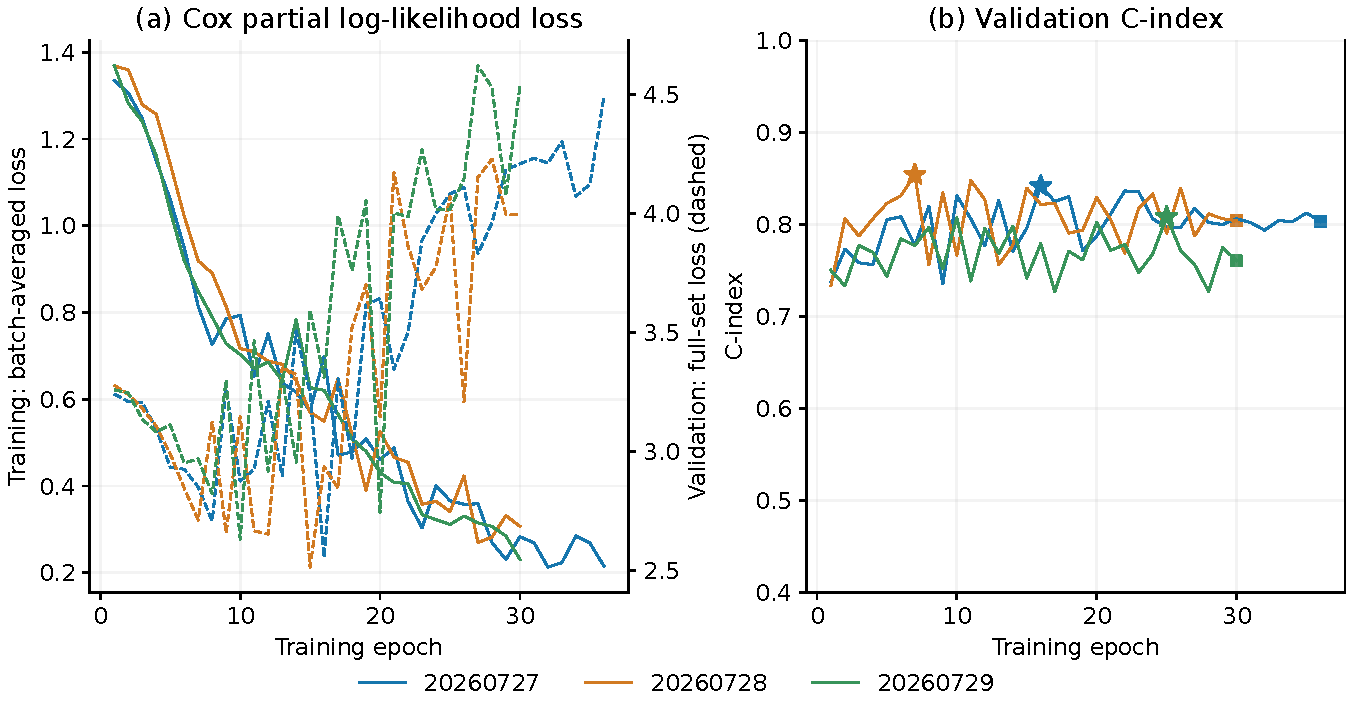
\includegraphics[width=\textwidth]{image_en/empirical-training.pdf}
\caption{Training convergence dynamics of RC-Free across three seeds}
\label{fig:empirical-training}
\captionsetup{justification=raggedright}
\caption*{Panel (a): batch-averaged training Cox loss (solid curves, left axis) and full-set validation Cox loss (dashed curves, right axis). Panel (b): validation C-index across epochs; star markers denote selected best checkpoints, and square markers denote early-stopping epochs.}
\end{figure}

The training trajectories in Figure~\ref{fig:empirical-training} demonstrate that across all three runs, the training loss decreases smoothly (from 1.33--1.37 down to 0.22--0.31), whereas the validation loss exhibits a gradual upward trend after the early epochs (from 3.24--3.28 to 3.99--4.53)---a classic signature of overfitting when optimizing deep neural networks on a modest clinical cohort. It is important to emphasize that the absolute magnitudes of the two loss axes should not be compared directly, because the Cox partial log-likelihood scales with the size of the risk set \cite{kvamme2019time} (at most 6 participants per training mini-batch versus all 54 participants on the full validation set). Because the primary objective of the task is risk ranking, I select the optimal checkpoint based on the peak validation C-index (Panel b): the three runs select checkpoints at epochs 16, 7, and 25 (achieving validation C-indices of 0.8417, 0.8542, and 0.8083, respectively) and trigger early stopping at epochs 36, 30, and 30.

\section{Longitudinal and Multimodal Ablation (RQ1--RQ2)}
First, to establish a solid empirical foundation, I conduct an exploratory ablation study addressing the first two research questions: whether longitudinal information from repeated MRI scans and the addition of radiomics and clinical scores genuinely improve risk-ranking concordance. Table~\ref{tab:exploratory} summarizes the validation C-index across progressively enriched input configurations (evaluated on seed 20260727).

\begin{table}[H]
\centering\small
\caption{Validation C-index across input configurations (seed 20260727).}
\label{tab:exploratory}
\begin{tabularx}{\linewidth}{@{}Y r@{}}
\toprule
\textbf{Model Configuration} & \textbf{C-index $\uparrow$} \\
\midrule
Last-MRI (single-timepoint baseline) & 0.7333 \\
Longitudinal MRI + T-LSTM & 0.7333 \\
Longitudinal MRI + T-LSTM + Attention & 0.7833 \\
Three-Modality Concatenation (MRI + Radiomics + Clinical) & \textbf{0.8125} \\
\bottomrule
\end{tabularx}
\end{table}

The empirical results reveal two distinct performance leaps. First, relying solely on the final hidden state of the T-LSTM over three MRI scans fails to outperform the single-timepoint Last-MRI baseline (both achieving 0.7333); however, once the additive attention mechanism is incorporated to aggregate all three visits with learned weights, the validation C-index jumps from 0.7333 to 0.7833 (+0.0500). This finding confirms that the prognostic value of longitudinal imaging is unlocked only when the model can adaptively balance contributions across visits rather than passively depending on the final recurrent state. Second, incorporating whole-brain radiomics and clinical assessment scores via simple feature concatenation further elevates the C-index to \textbf{0.8125} (+0.0292 over the best MRI-only configuration). Building upon this clear empirical evidence, all subsequent architectural experiments retain all three input modalities together with the T-LSTM and additive attention backbone.

\section{Concatenation vs. Outer-Product (RQ3)}
\label{sec:matched-fusion}
Having confirmed the indispensable contribution of all three longitudinal modalities, I next investigate the third research question (RQ3): whether explicitly modeling bilinear pairwise interactions via the outer product outperforms traditional feature concatenation. To strictly isolate the pure effect of the fusion mechanism, I hold all other architectural components fixed (including the 3D ResNet-18 backbone, 128-dimensional T-LSTM, additive attention, Breslow Cox objective, and all training hyperparameters) and ensure \emph{identical initial weights} for all shared modules across each random seed (Table~\ref{tab:matched-fusion}).

\begin{table}[H]
\centering\small
\caption{Validation C-index of Concatenation vs. Full Outer-Product (mean $\pm$ SD).}
\label{tab:matched-fusion}
\begin{tabularx}{\linewidth}{@{}Y r@{}}
\toprule
\textbf{Fusion Architecture} & \textbf{C-index $\uparrow$} \\
\midrule
Concatenation & $0.8149\pm0.0214$ \\
Full Outer-Product & $\mathbf{0.8285\pm0.0272}$ \\
\bottomrule
\end{tabularx}
\end{table}

Under strictly matched initialization conditions, the Full Outer-Product variant achieves a mean validation C-index of \textbf{0.8285}, outperforming the 0.8149 achieved by standard feature concatenation (a mean gain of \textbf{0.0135} computed on unrounded values). This consistent improvement demonstrates that explicitly constructing second-order cross-products enables the neural network to exploit inter-modality relationships more effectively. This finding establishes Full Outer-Product as the reference starting point for two subsequent architectural refinements: compressing interaction parameters via CP decomposition and pruning redundant pairwise interactions.

\section{CP Compression and Topology Search (RQ4--RQ5)}
\label{sec:cp-results}
\label{sec:ablation-results}
\label{sec:rcfree-multiseed}
\label{sec:standardized-benchmark}
\label{sec:paper-adaptation-results}

Starting from the Full Outer-Product architecture, I perform two controlled simplification steps across the same three random seeds (20260727--20260729), and subsequently benchmark the resulting architecture against the adapted CNN--PCA--T-LSTM reference pipeline to address RQ4 and RQ5.

\subsection{Parameter Reduction via CP Decomposition (RQ4)}
\label{sec:computational-efficiency}
When transitioning from Full Outer-Product to Full CP, all modality encoders, gated residual routing branches, and downstream temporal modules remain completely unchanged; the sole modification is that the initial bilinear layer of the three pairs (MR, MC, and RC) is parameterized via CP decomposition with ranks 8, 8, and 4, respectively (Table~\ref{tab:cpconfig}). Table~\ref{tab:interaction-parameters} compares the resulting parameter counts across three distinct architectural scopes.

\begin{table}[H]
\centering\small
\caption{Parameter counts of Full Outer-Product and Full CP across scopes.}
\label{tab:interaction-parameters}
\begin{tabularx}{\linewidth}{@{}Y r r@{}}
\toprule
\textbf{Architectural Scope} & \textbf{Full Outer-Product} & \textbf{Full CP} \\
\midrule
Three initial bilinear layers & 229696 & \textbf{3712} \\
Three complete interaction blocks (including MLPs) & 248608 & \textbf{22624} \\
Entire network & 33760941 & \textbf{33534957} \\
\bottomrule
\end{tabularx}
\end{table}

The figures in Table~\ref{tab:interaction-parameters} highlight the dramatic local compression achieved by CP decomposition: across the three initial bilinear layers, the number of learnable parameters drops from 229696 down to just 3712, representing a \textbf{98.38\% reduction}; when accounting for the entire interaction blocks (including their downstream MLPs), the parameter reduction remains an impressive \textbf{90.90\%}. By contrast, at the whole-network scale, the relative reduction is approximately 0.67\% because the 3D ResNet-18 backbone of the MRI branch dominates the total parameter budget and remains unchanged. In exchange for this substantial structural compression at the interaction layer, the mean validation C-index of Full CP (0.8278) trails Full Outer-Product (0.8344) by only a minor margin of 0.0066 on the main benchmark suite (Table~\ref{tab:standard-bench}). Rather than stopping at Full CP, the next step examines whether pruning redundant pairwise interactions can simultaneously save additional parameters and fully recover ranking concordance.

\subsection{Seven-Topology Benchmark and RC-Free (RQ5)}
\label{sec:new-topology}
To test the hypothesis that retaining all three pairwise interactions is unnecessary, I systematically evaluate all seven CP topologies containing at least one active interaction pair (comprising three single-pair variants, three two-pair variants, and the three-pair Full CP model). Crucially, \emph{every topology retains all three input modalities and their direct representation pathways}; the only difference lies in which pairwise bilinear interactions are activated. Table~\ref{tab:new-topology} reports the empirical results across the three random initializations.

\begin{table}[H]
\centering\small
\caption{Parameters and validation C-index across seven CP topologies (mean $\pm$ SD).}
\label{tab:new-topology}
\begin{tabularx}{\linewidth}{@{}Y c r r@{}}
\toprule
\textbf{Topology} & \textbf{Pairs / routes} & \textbf{Parameters} & \textbf{C-index $\uparrow$} \\
\midrule
MR-only & 1 / 2 & 33484165 & $0.8299\pm0.0267$ \\
MC-only & 1 / 2 & 33484037 & $0.8236\pm0.0237$ \\
RC-only & 1 / 2 & 33464165 & $0.8319\pm0.0214$ \\
RC-Free (MR+MC) & 2 / 4 & 33519497 & $\mathbf{0.8347\pm0.0237}$ \\
MR-Free (MC+RC) & 2 / 4 & 33499625 & $0.8243\pm0.0249$ \\
MC-Free (MR+RC) & 2 / 4 & 33499753 & $0.8222\pm0.0156$ \\
Full CP & 3 / 6 & 33534957 & $0.8278\pm0.0250$ \\
\bottomrule
\end{tabularx}
\end{table}

Across all seven surveyed topologies, \textbf{RC-Free (MR+MC)} achieves the highest mean validation C-index (\textbf{0.8347}), followed by the single-pair RC-only configuration (0.8319). Notably, compared with Full CP, omitting the direct RC interaction reduces the number of gated residual branches from six to four, \textbf{saves 15460 parameters}, and elevates the mean validation C-index from 0.8278 to 0.8347. Considering domain-grounded architectural design (positioning MRI as the central hub), ranking accuracy, and parameter compactness together, RC-Free emerges as the optimal architecture for in-depth survival stratification analysis.

\subsection{Overall Comparison Against the Reference Pipeline}
Table~\ref{tab:standard-bench} benchmarks the proposed RC-Free model against Full Outer-Product, Full CP, and the adapted re-implementation of the CNN--PCA--T-LSTM pipeline of Aghajanian et al. on the same validation set.

\begin{table}[H]
\centering\small
\caption{Validation C-index across benchmark models (mean $\pm$ SD).}
\label{tab:standard-bench}
\begin{tabularx}{\linewidth}{@{}Y r r c@{}}
\toprule
\textbf{Model} & \textbf{C-index $\uparrow$} & \textbf{Parameters} & \textbf{Pairs / routes} \\
\midrule
CNN--PCA--T-LSTM & $0.7417\pm0.0693$ & $33213122$ & 0 / 0 \\
Full Outer-Product & $0.8344\pm0.0148$ & $33760941$ & 3 / 6 \\
Full CP Pairwise & $0.8278\pm0.0250$ & $33534957$ & 3 / 6 \\
RC-Free Pairwise & $\mathbf{0.8347\pm0.0237}$ & $33519497$ & 2 / 4 \\
\bottomrule
\end{tabularx}
\caption*{\textit{Note.} All figures in this table are evaluated on the same validation set. The reference CNN--PCA--T-LSTM model follows the pipeline of Aghajanian et al.~\cite{aghajanian2025longitudinal} with the adaptations summarized in Table~\ref{tab:reference-methods}.}
\end{table}


Compared with Full Outer-Product, the RC-Free architecture \textbf{reduces 241444 parameters} (streamlining from 3 pairs / 6 routes down to 2 pairs / 4 routes) while achieving the highest mean validation C-index (\textbf{0.8347} versus 0.8344). More importantly, when benchmarked against the CNN--PCA--T-LSTM reference pipeline ($0.7417\pm0.0693$), all three end-to-end multimodal fusion architectures outperform the reference baseline by approximately 0.086 to 0.093 C-index points, while reducing cross-seed standard deviation by nearly threefold (0.0148--0.0250 versus 0.0693). This result demonstrates that end-to-end training combining a pretrained 3D volumetric encoder with explicit cross-modal interactions delivers superior ranking concordance and numerical stability compared with a decoupled two-stage pipeline relying solely on PCA-compressed imaging features.

\section{Survival Analysis of the RC-Free Model}
\label{sec:posthoc-test}
\label{sec:survival-results}
With the optimal RC-Free architecture selected, this section conducts an in-depth evaluation of the estimated log-risk scores $\eta_i$ across both the validation set (primary evaluation) and the held-out post-hoc test set from two complementary perspectives: horizon-specific discrimination (IPCW-AUC) and longitudinal risk-group stratification (Kaplan--Meier curves).

\subsection{C-index and Time-Dependent AUC at 2, 3, and 5 Years}
Table~\ref{tab:survival-metrics} summarizes the global C-index alongside the time-dependent IPCW-AUC values at three clinical horizons, accompanied by Table~\ref{tab:horizon-support} reporting the exact counts of cumulative cases, dynamic controls, and right-censored subjects at each horizon to clarify the sample support underlying each estimate.

\begin{table}[H]
\centering\small
\caption{C-index and IPCW time-dependent AUC of RC-Free (mean $\pm$ SD).}
\label{tab:survival-metrics}
\begin{tabularx}{\linewidth}{@{}Y r r@{}}
\toprule
\textbf{Metric} & \textbf{Validation (primary)} & \textbf{Test (post-hoc)} \\
\midrule
C-index & $\mathbf{0.8347\pm0.0237}$ & $\mathbf{0.8466\pm0.0267}$ \\
2-year AUC & $\mathbf{0.9805\pm0.0149}$ & $0.8858\pm0.0245$ \\
3-year AUC & $\mathbf{0.9788\pm0.0162}$ & $0.8770\pm0.0318$ \\
5-year AUC & $0.7889\pm0.0632$ & $0.8483\pm0.0508$ \\
\bottomrule
\end{tabularx}
\caption*{\textit{Note.} Each evaluation split comprises 54 participants with 16 observed events across three random initializations.}
\end{table}

\begin{table}[H]
\centering\small
\caption[Participant counts by outcome status and uncensored survival probability at each horizon]{At each horizon, the three counts denote cumulative cases up to the horizon, dynamic controls remaining under follow-up beyond the horizon, and subjects right-censored at or before the horizon, respectively. The uncensored probability $\widehat G(h)$ is estimated from the training set.}
\label{tab:horizon-support}
\begin{tabularx}{\linewidth}{@{}c Y Y r@{}}
\toprule
\textbf{Horizon (years)} & \textbf{Validation} & \textbf{Test (post-hoc)} & \textbf{$\widehat G(h)$} \\
\midrule
2 & 7 / 37 / 10 & 8 / 37 / 9 & $0.831$ \\
3 & 7 / 34 / 13 & 11 / 29 / 14 & $0.697$ \\
5 & 12 / 19 / 23 & 14 / 16 / 24 & $0.475$ \\
\bottomrule
\end{tabularx}
\end{table}


On the validation set, RC-Free achieves strong discrimination at the earlier horizons, recording an AUC of \textbf{0.9805} at 2 years and \textbf{0.9788} at 3 years, before decreasing to 0.7889 at the 5-year horizon. Cross-referencing with the sample support in Table~\ref{tab:horizon-support} reveals that this trajectory directly reflects the underlying sample structure at each time point. At the 2- and 3-year horizons, the validation set contains only \textbf{7 cumulative cases}, meaning that finite-sample variability is naturally non-negligible. By the 5-year horizon, although the number of cumulative cases increases to 12, the number of dynamic controls remaining under active follow-up beyond 5 years drops sharply from 37 down to 19 due to 23 subjects being right-censored earlier. Figure~\ref{fig:empirical-roc} visually reflects this phenomenon: at the 5-year validation horizon, the ROC curves across the three seeds exhibit wider dispersion (SD increasing to 0.0632) compared with the tight clustering at the 2- and 3-year horizons. Reassuringly, on the independent post-hoc test set, discrimination remains highly consistent across all three horizons (achieving AUCs of 0.8858, 0.8770, and 0.8483 at 2, 3, and 5 years, respectively), accompanied by an overall C-index of $0.8466\pm0.0267$.

\begin{figure}[H]
\centering
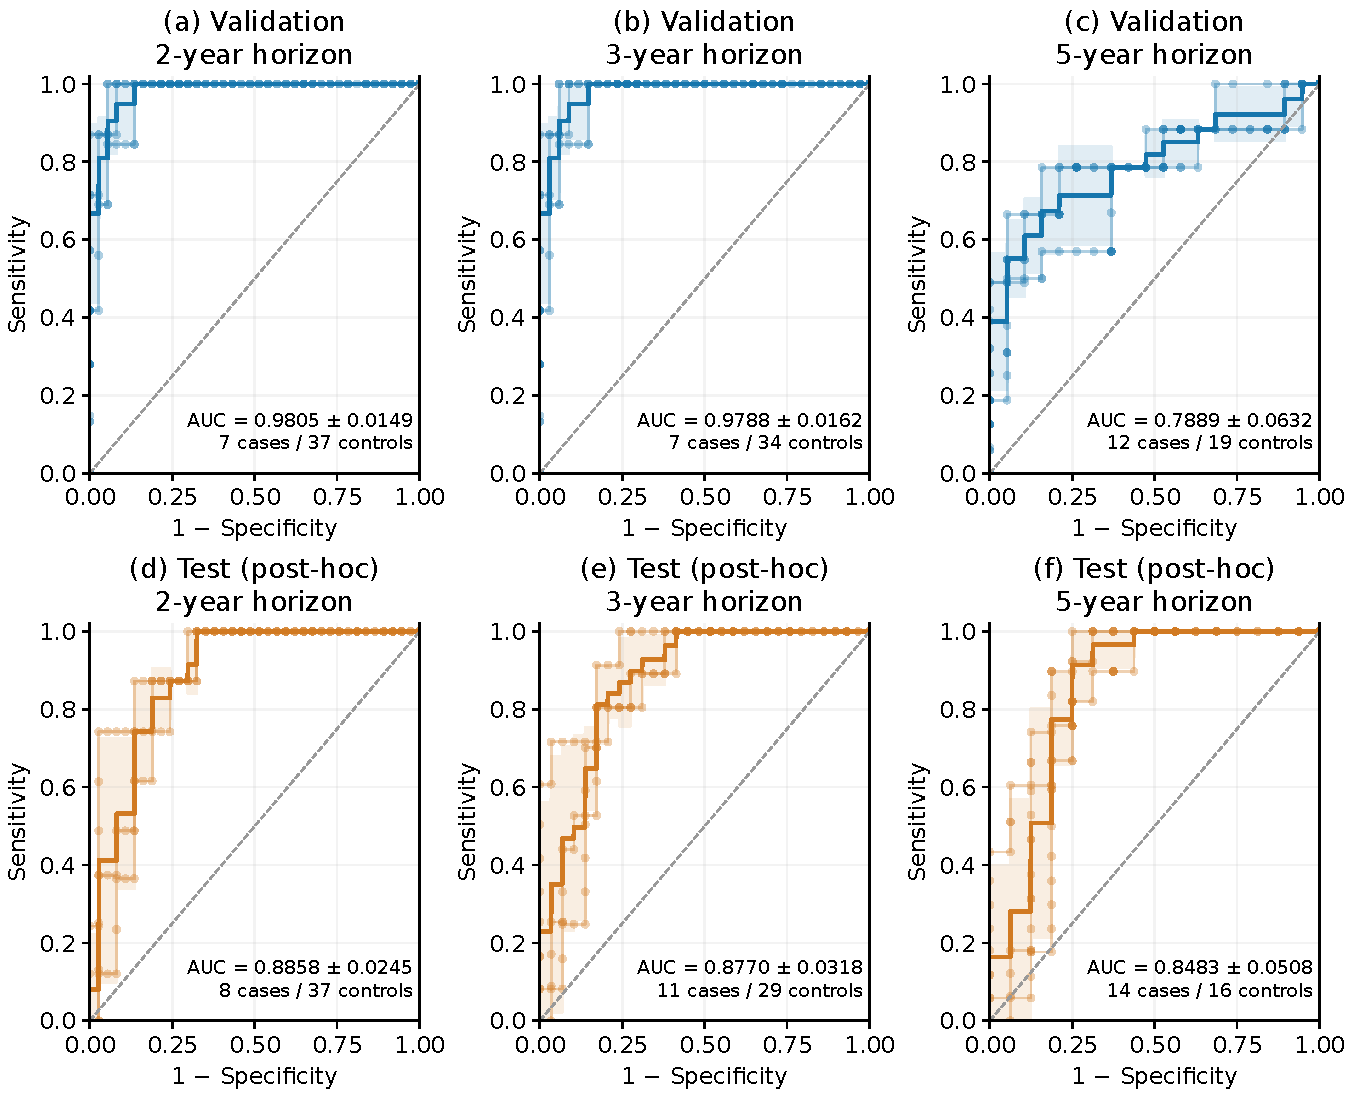
\includegraphics[width=\textwidth,trim=0bp 263.8bp 0bp 0bp,clip]{image_en/empirical-ipcw-roc.pdf}\\[3.6cm]
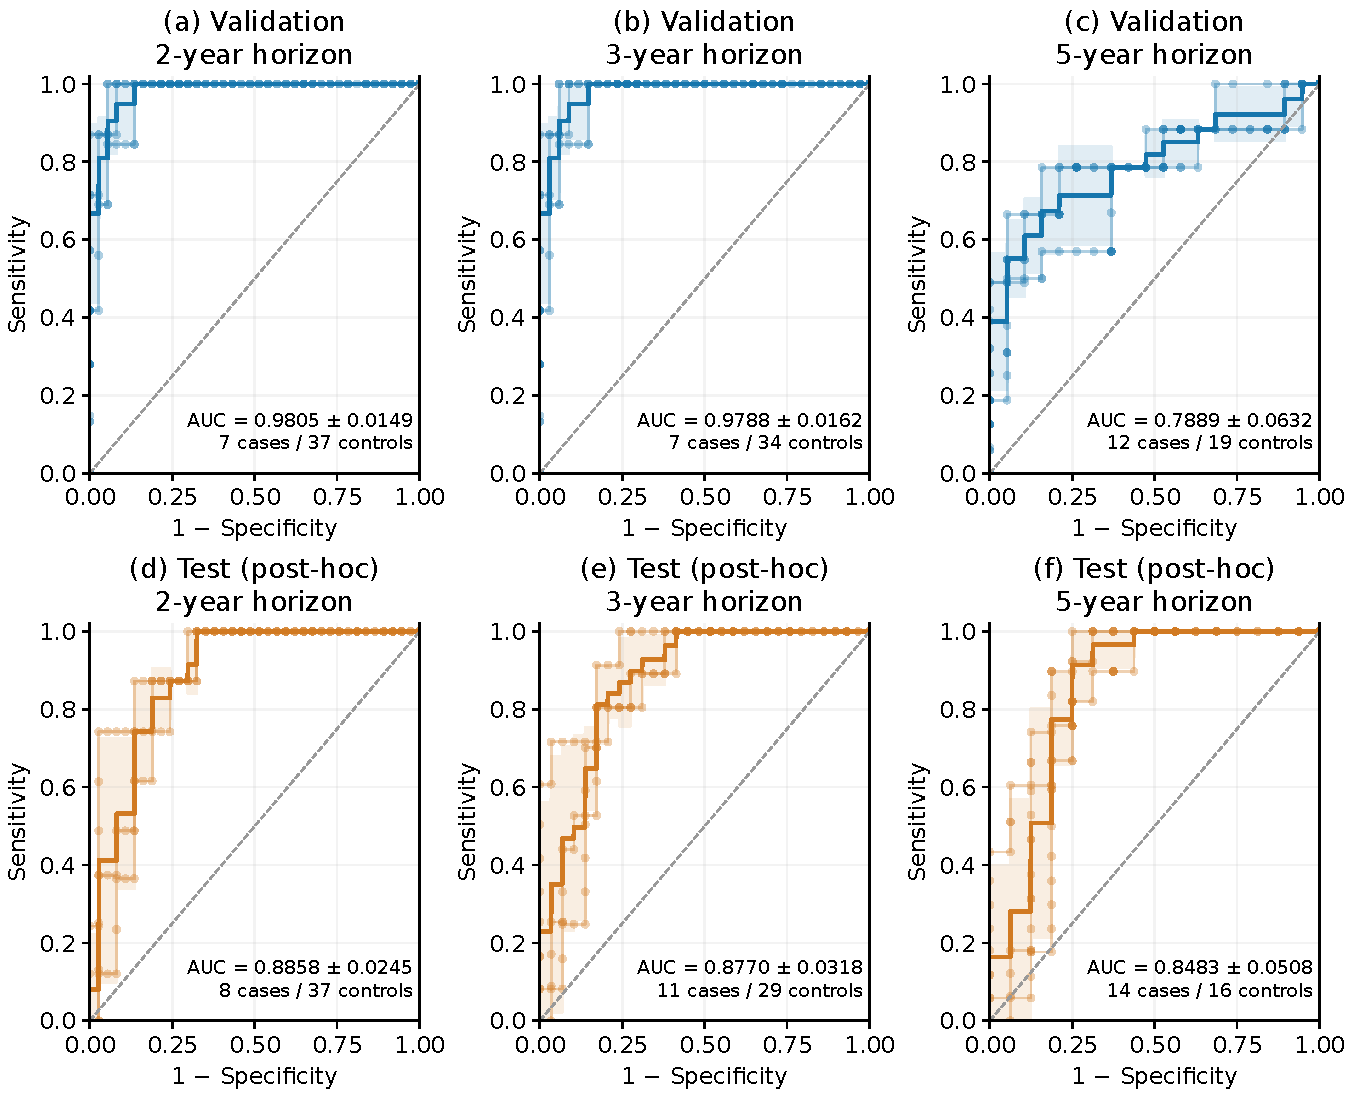
\includegraphics[width=\textwidth,trim=0bp 0bp 0bp 263.0bp,clip]{image_en/empirical-ipcw-roc.pdf}
\caption{IPCW time-dependent ROC curves of RC-Free at 2, 3, and 5 years}
\label{fig:empirical-roc}
\captionsetup{justification=raggedright}
\caption*{Top row: validation set; bottom row: post-hoc test set. Thin curves and circular markers represent individual seeds; bold curves denote the across-seed mean; shaded bands indicate $\pm1$ SD. The diagonal dashed line represents random guessing.}
\end{figure}

\clearpage
\subsection{Kaplan--Meier Stratification via Consensus Risk Groups}
Figure~\ref{fig:survival-km} and Table~\ref{tab:km-statistics} evaluate the model's ability to stratify participants into high- and low-risk progression groups (defined using the fixed training-set median risk cutoff and majority-vote consensus across the three random initializations).

\begin{figure}[H]
\centering
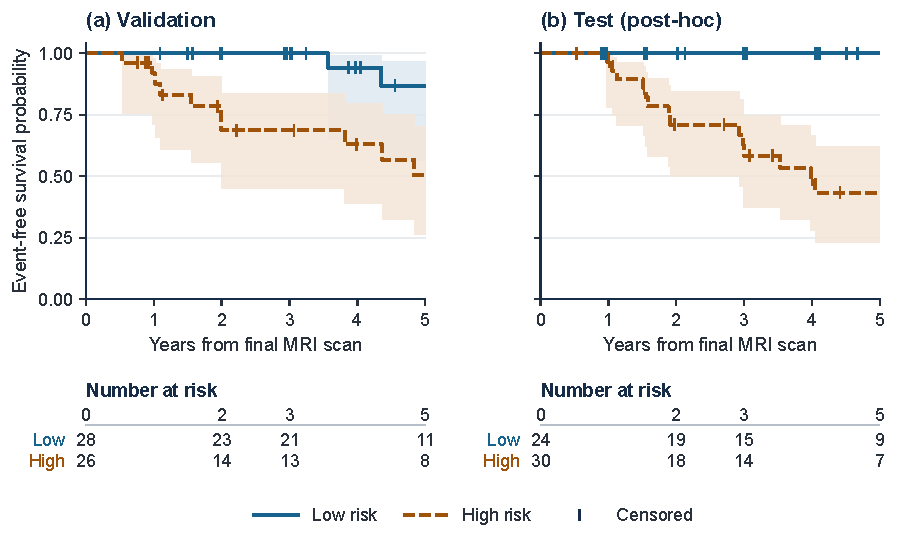
\includegraphics[width=\textwidth]{image_en/survival-km.pdf}
\caption{Kaplan--Meier survival curves across RC-Free risk groups}
\label{fig:survival-km}
\captionsetup{justification=raggedright}
\caption*{Panel (a): validation set; Panel (b): post-hoc test set. Shaded bands represent 95\% confidence intervals; vertical tick marks indicate right-censoring times. The tables below the horizontal axes report the number of subjects remaining at risk at each time horizon.}
\end{figure}

\begin{table}[H]
\centering\small
\caption{Log-rank test, hazard ratio (HR), and PH assumption test.}
\label{tab:km-statistics}
\begin{tabularx}{\linewidth}{@{}Y r r r r@{}}
\toprule
\textbf{Dataset split} & \textbf{Log-rank $p$} & \textbf{HR} & \textbf{95\% CI} & \textbf{$p$ (PH)} \\
\midrule
Validation & $\mathbf{0.0134}$ & $\mathbf{3.79}$ & $1.22$--$11.78$ & $0.1031$ \\
Test (post-hoc) & $\mathbf{<0.001}$ & $\mathbf{16.17}$ & $2.12$--$123.17$ & $0.1592$ \\
\bottomrule
\end{tabularx}
\end{table}


The two survival curves separate clearly across both dataset splits, confirming the strong risk-stratification capability of the proposed model. On the validation set, the low-risk group (28 participants) records only 4 progression events, whereas the high-risk group (26 participants) experiences 12 progression events---three times as many as the low-risk group; the log-rank test confirms statistically significant separation (\textbf{$p=0.0134$}), with an estimated hazard ratio of \textbf{HR = 3.79} (95\% CI: 1.22--11.78). On the post-hoc test set, the separation is even more pronounced: among the 24 participants assigned to the low-risk group, virtually no cognitive progression occurs during the first 5 years of follow-up (with only a single event recorded after year 5), in stark contrast to 15 progression events among the 30 participants in the high-risk group, yielding \textbf{log-rank $p<0.001$} and \textbf{HR = 16.17} (95\% CI: 2.12--123.17). The wide confidence interval of the hazard ratio on the test set arises directly from the fact that the low-risk reference group contains only a single event in the denominator; even so, the lower bound of the 95\% confidence interval still reaches 2.12, confirming a substantially elevated progression rate in the high-risk group. Furthermore, the Schoenfeld residuals test yields $p=0.1031$ on the validation set and $p=0.1592$ on the test set (both exceeding 0.05), indicating no evidence against the proportional hazards assumption over time and confirming that RC-Free delivers both accurate global ranking and reliable longitudinal survival stratification.

\section{Answers to the Research Questions}
\label{sec:rq-results}
Synthesizing the empirical investigations presented throughout this chapter, the five research questions posed in Table~\ref{tab:rq} are restated and answered in detail below:

\begin{description}[leftmargin=1.35cm,labelwidth=1.1cm,itemsep=.4em]
\item[RQ1.] \emph{Do longitudinal multi-timepoint MRI scans provide superior risk discrimination compared with using only the final MRI scan?} Yes, provided that the visit sequence is aggregated via adaptive attention. Relying solely on the final T-LSTM state matches the single-scan \emph{Last-MRI} baseline (validation C-index 0.7333), whereas adding additive attention across all three irregularly spaced visits raises the C-index to \textbf{0.7833} (+0.0500, Table~\ref{tab:exploratory}), capturing within-person atrophy dynamics.
\item[RQ2.] \emph{Does incorporating radiomics and clinical scores improve risk discrimination over using MRI alone?} Yes. Adding whole-brain PyRadiomics descriptors (16 PCA components) and clinical MMSE/CDR assessments (9 scores with 9 missingness indicators) elevates the validation C-index from 0.7833 to \textbf{0.8125} (+0.0292, Table~\ref{tab:exploratory}), confirming complementary value across macroscopic anatomy, tissue texture statistics, and cognitive-functional scales.
\item[RQ3.] \emph{Is pairwise bilinear interaction more effective than simple feature concatenation?} Yes. Under matched initial weights for all shared modules across three random seeds, \emph{Full Outer-Product} fusion achieves a mean validation C-index of \textbf{0.8285} versus 0.8149 for \emph{Concatenation}---a mean gain of \textbf{0.0135} on unrounded values (Table~\ref{tab:matched-fusion})---by explicitly modeling second-order cross-modal products through gated residual routes.
\item[RQ4.] \emph{How many interaction-layer parameters does CP decomposition reduce, and how does it affect the C-index?} Low-rank CP factorization ($Q=8$ for MR and MC; $Q=4$ for RC) reduces the three initial bilinear layers by \textbf{98.38\%} (from 229696 to 3712 parameters) and the three complete interaction blocks by \textbf{90.90\%} (0.67\% whole-network reduction, Table~\ref{tab:interaction-parameters}), while incurring only a minor 0.0066 difference in mean validation C-index between \emph{Full CP} (0.8278) and \emph{Full Outer-Product} (0.8344, Table~\ref{tab:standard-bench}).
\item[RQ5.] \emph{Can redundant pairwise interactions be pruned while preserving risk discrimination performance?} Yes---pruning the direct RC pair while keeping MRI as the central hub in \textbf{RC-Free (MR+MC)} reduces gated routes from six to four, saves \textbf{15460 parameters} over \emph{Full CP} (241444 over \emph{Full Outer-Product}), and attains the highest mean validation C-index among all seven CP topologies (\textbf{0.8347}, Table~\ref{tab:new-topology}; post-hoc test \textbf{0.8466}, Table~\ref{tab:survival-metrics}), with significant Kaplan--Meier separation on validation ($p=0.0134$, $\mathrm{HR}=3.79$) and post-hoc test ($p<0.001$, $\mathrm{HR}=16.17$, Table~\ref{tab:km-statistics}).
\end{description}

\chapter[Discussion, Conclusion, and Future Work]{Discussion, Conclusion,\\and Future Work}
\label{chap:discussion}

\section{Discussion of Principal Findings}
Synthesizing the empirical results presented in Chapter~\ref{chap:results}, this thesis distills three key architectural lessons for multimodal deep survival analysis on modest-sized clinical cohorts:

First, \emph{the parameter-compression efficiency of CP decomposition must be evaluated within its specific architectural scope}. Replacing full outer-product projection layers with low-rank CP factorization reduces the parameter count of the three initial bilinear layers by \textbf{98.38\%} (from 229696 down to just 3712 parameters) and achieves a 90.90\% reduction across the complete interaction blocks including their downstream MLPs. However, this translates to an overall whole-network reduction of approximately 0.67\% because the 3D ResNet-18 volumetric encoder dominates the total parameter budget. This distinction clarifies that the primary benefit of applying CP decomposition in this architecture lies not in shrinking overall model storage size, but rather in \emph{preventing localized overfitting at the multimodal fusion bottleneck}---the exact location most vulnerable to parameter explosion when combining multiple feature streams on a training cohort of only 251 patients. The minor 0.0066 C-index trade-off between Full CP and Full Outer-Product represents a highly reasonable price for structural regularization at the interaction layer.

Second, \emph{activating more pairwise interactions does not automatically yield superior prognostic performance}. Across all seven surveyed CP architectures containing at least one pairwise interaction, the proposed RC-Free topology retains only the two MRI-centered interaction pairs (MR and MC) with four gated residual branches, yet achieves the highest mean validation C-index (\textbf{0.8347}). This result not only surpasses the three-pair Full CP model (0.8278) while saving 15460 parameters, but even the single-pair RC-only configuration reaches 0.8319, outperforming Full CP. The underlying reason is that all three input modalities already preserve their direct representation pathways through gated residual connections; consequently, forcing all three pairwise interactions simultaneously can introduce representational redundancy and increase estimation variance on a limited cohort. By positioning 3D structural MRI as the central hub connecting whole-brain radiomics and clinical scores, RC-Free provides the most balanced, compact, and effective fusion topology.

Third, \emph{the practical interpretation of risk stratification is inherently linked to sample size and cumulative event counts}. Kaplan--Meier survival analysis confirms that the log-risk scores generated by RC-Free separate patients into distinct progression trajectories, achieving log-rank $p=0.0134$ on the validation set (12/26 events in the high-risk group versus 4/28 in the low-risk group) and $p<0.001$ on the independent post-hoc test set. Nevertheless, when examining horizon-specific discrimination, the high validation AUCs at 2 and 3 years (0.9805 and 0.9788) rely on only \textbf{7 cumulative events}. By the 5-year horizon, the validation AUC decreases to 0.7889 with wider cross-seed standard deviation as the number of event-free subjects remaining under active follow-up beyond 5 years drops to 19 (Table~\ref{tab:horizon-support}).

\section{Study Limitations}
\label{sec:study-limitations}
Despite encouraging empirical results, this thesis acknowledges four methodological limitations:
\begin{enumerate}[itemsep=0.15em,topsep=0.25em]
\item \textbf{Data are currently restricted to the international ADNI cohort and have not yet been validated in Vietnamese hospitals.} All training, hyperparameter tuning, and testing in this study rely exclusively on the international ADNI database with modest evaluation split sizes (54 validation and 54 post-hoc test participants). The model has not yet been collected or externally validated on real-world patient cohorts from major hospitals in Vietnam, where MRI scanner protocols, clinical workflow practices, and demographic profiles may differ substantially.
\item \textbf{Retrospective time-axis design.} The survival time $t_i$ is measured from the third MRI scan date $p_i$, whereas the cohort inclusion criteria require participants to remain event-free through the 18-month milestone $L_i$ (creating potential immortal time bias if the model were interpreted as a prospective forecasting tool deployed immediately at scan date $p_i$ \cite{suissa2008immortal}). In addition, the $\pm90$-day clinical matching window results in 57 participants having an MMSE or CDR score linked to their third MRI scan that was actually recorded after date $p_i$ (Section~\ref{sec:data-split}), making the current findings strictly suited for retrospective evaluation on the stable post-$L_i$ cohort.
\item \textbf{Input predictors and outcome event criteria both rely on MMSE and CDR.} Although the input observation window and post-milestone outcome window are chronologically separated around the 18-month mark, defining progression events via MMSE and CDR thresholds inevitably couples the outcome definition to these two rating scales; the model has not yet been evaluated against independent specialist clinical diagnoses or pathological fluid/PET biomarkers.
\item \textbf{Model output is currently limited to relative risk ranking.} The scalar log-risk score $\eta_i$ from the Cox head establishes who is at higher risk of earlier progression relative to other patients, but has not yet been calibrated into an individualized absolute progression probability (in percentage terms at specific clinical horizons), nor has real-time inference latency been benchmarked on hospital workstation hardware.
\end{enumerate}

\section{Future Work}
Building directly upon the limitations identified above, I propose three practical directions for future research:
\begin{enumerate}[itemsep=0.15em,topsep=0.25em]
\item \emph{External validation on real-world hospital cohorts in Vietnam}: Collaborating with major domestic hospitals to collect longitudinal follow-up data from Vietnamese patients, evaluate external generalizability, adapt the model to local clinical settings, and incorporate readily available domestic laboratory markers.
\item \emph{Refining the temporal landmark prediction design}: Enforcing a strict cutoff ensuring that all input clinical assessments occur prior to the final MRI scan date $p_i$, or adopting a strict fixed-landmark survival design starting from milestone $L_i$ \cite{vanhouwelingen2007dynamic} to completely eliminate temporal overlap between input observations and outcome follow-up.
\item \emph{Calibrating individualized progression probabilities and enhancing clinical interpretability}: Estimating the baseline survival function via Breslow's estimator \cite{kvamme2019time} to convert relative log-risk scores into calibrated annual progression probabilities for individual patients, while analyzing learned attention weights and dynamic gating coefficients to provide transparent explanations and benchmarking inference runtime for clinical deployment.
\end{enumerate}

\section{Conclusion}
Prognosticating disease progression among individuals with mild cognitive impairment (MCI) requires not only tracking longitudinal disease trajectories across repeated clinical visits, but also harmonizing brain structural morphology, quantitative mathematical texture descriptors, and clinical cognitive assessments. Using a retrospective cohort of 359 participants from the ADNI initiative across three longitudinal visits, this thesis has developed an end-to-end multimodal deep survival analysis pipeline integrating 3D structural MRI volumes, whole-brain radiomics features, and clinical MMSE/CDR scores. Systematic ablation experiments confirm the contribution of each architectural design step: longitudinal MRI sequences modeled with T-LSTM and additive attention substantially outperform single-timepoint scans; integrating all three modalities markedly elevates risk-ranking concordance; and explicitly modeling pairwise bilinear interactions captures cross-modal relationships more effectively than standard feature concatenation.

Notably, the proposed \textbf{RC-Free} architecture combines two complementary simplification mechanisms: low-rank CP tensor decomposition reduces the parameter count of the three initial bilinear layers by 98.38\%, and pruning the direct RC interaction saves an additional 15460 parameters relative to Full CP while retaining all three input sources. On the validation set, RC-Free achieves the highest mean C-index among all seven pairwise CP topologies ($0.8347\pm0.0237$) and delivers statistically significant survival group separation on Kaplan--Meier curves ($p=0.0134$). Together, these findings demonstrate that combining low-rank tensor parameterization with domain-informed interaction pruning offers a compact, accurate, and promising paradigm for multimodal survival prognosis on sample-limited clinical datasets.

\clearpage
\appendix
\begingroup
\renewcommand{\chaptername}{Appendix}
\titleformat{\chapter}[hang]{\normalfont\bfseries\Large}{\chaptername\ \thechapter.}{0.5em}{}
\titlespacing*{\chapter}{0pt}{0pt}{12pt}
\addtocontents{toc}{\protect\renewcommand{\protect\cftchappresnum}{Appendix~}}

\begin{landscape}
\chapter{Comprehensive Master Schematic of the RC-Free Pipeline}
\label{app:master-pipeline}
\begin{figure}[H]
\centering
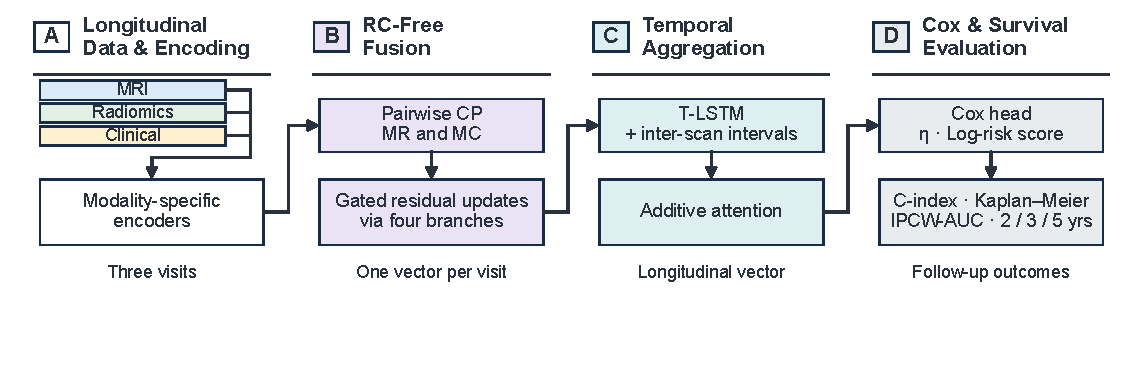
\includegraphics[width=\linewidth,height=11.5cm,keepaspectratio]{image_en/master-pipeline.pdf}
\caption{End-to-end master schematic of the RC-Free pipeline from raw inputs to survival evaluation}
\label{fig:master-pipeline}
\end{figure}
\end{landscape}

\clearpage
\chapter{Feature Map Dimensions of the 3D MRI Encoder}
\label{app:mri-shapes}
Table~\ref{tab:mri-encoder-shapes} details the intermediate feature map dimensions across each stage of the 3D ResNet-18 MRI encoder (implemented in MONAI version 1.5.2 and initialized from MedicalNet pretrained weights \cite{chen2019med3d,cardoso2022monai}). Each 3D feature map has shape $[B, C_{\mathrm{ch}}, D, H, W]$, where $B$ denotes the batch size, $C_{\mathrm{ch}}$ denotes the number of channels, and $D, H, W$ represent the three spatial dimensions. All three visits of a participant share this encoder; following global average pooling, the three 512-dimensional vectors are stacked along the temporal axis into $[B, 3, 512]$ before being linearly projected to $M_t\in\mathbb R^{128}$.

\begin{table}[H]
\centering
\small
\caption[Feature map dimensions of the 3D ResNet-18 encoder]{Feature map dimensions across layers of the 3D ResNet-18 volumetric encoder}
\label{tab:mri-encoder-shapes}
\begin{tabularx}{\textwidth}{@{}Y l@{}}
\toprule
\textbf{Stage / Operation} & \textbf{Output Shape} \\
\midrule
Input 3D MRI volume & $[B,1,144,144,144]$ \\
$7^3$ 3D convolution, stride 1, padding 3; BN; ReLU & $[B,64,144,144,144]$ \\
$3^3$ max pooling, stride 2, padding 1 & $[B,64,72,72,72]$ \\
ResNet Stage 1: two BasicBlocks & $[B,64,72,72,72]$ \\
ResNet Stage 2: first block stride 2 & $[B,128,36,36,36]$ \\
ResNet Stage 3: first block stride 2 & $[B,256,18,18,18]$ \\
ResNet Stage 4: first block stride 2 & $[B,512,9,9,9]$ \\
Global average pooling and flattening & $[B,512,1,1,1]\to[B,512]$ \\
Temporal stacking across the three visits & $[B,3,512]$ \\
Linear projection $512\to128$; GELU; Dropout 0.20; LayerNorm & $[B,3,128]$ \\
\bottomrule
\end{tabularx}
\end{table}

\endgroup


\clearpage
\phantomsection
\addcontentsline{toc}{chapter}{REFERENCES}
\renewcommand{\bibname}{REFERENCES}
\begingroup
\renewcommand{\bibfont}{\renewcommand{\baselinestretch}{1.15}\fontsize{12}{14}\selectfont}
\setlength{\bibsep}{0pt}
\bibliographystyle{thesisrefs}
\bibliography{references}
\endgroup

\end{document}
